\documentclass[conference]{IEEEtran}
\IEEEoverridecommandlockouts
% The preceding line is only needed to identify funding in the first footnote. If that is unneeded, please comment it out.
\usepackage{cite}
\usepackage{amsmath,amssymb,amsfonts}
\usepackage{algorithmic}
\usepackage{graphicx}
\usepackage{listings}
\lstset{breaklines=true}
\usepackage{url}
\usepackage{hyperref}
\usepackage{dirtree}
\graphicspath{ {images/} }
\usepackage{textcomp}
\usepackage{xcolor}
\usepackage{todonotes}
\usepackage{subcaption}
\usepackage{placeins}
\usepackage{comment}
\usetikzlibrary{positioning}

\usepackage{tikz}
\usetikzlibrary{calc, patterns, patterns.meta, shapes.geometric, arrows.meta, positioning, fit, decorations.pathreplacing, trees, arrows, shapes.misc, angles, quotes}
%Go-kart command \gokart{"x"}{"y"}{"rot_in_deg"}
\def\gokart#1#2#3{
    \begin{scope}[shift={(#1,#2)}, rotate=#3]
        \begin{scope}[shift={(0,-0.85)}] %Offset so (x,y) is the front bumper
            %Front bumper
            \draw[very thick] (-0.7, 0.75) -- (-0.5, 0.85) -- (0.5, 0.85) -- (0.7, 0.75);
            %Body
            \draw[fill=gray!30] (-0.5,-0.75) rectangle (0.5,0.75);
            %Wheels
            \draw[fill=black, rounded corners=0.75] (-0.6,0.6) rectangle (-0.4, 0.3); % Front left
            \draw[fill=black, rounded corners=0.75] (0.6,0.6) rectangle (0.4, 0.3); % Front right
            \draw[fill=black, rounded corners=0.75] (-0.6,-0.6) rectangle (-0.4, -0.3); % Rear left
            \draw[fill=black, rounded corners=0.75] (0.6,-0.6) rectangle (0.4, -0.3); % Rear right
            %Rear bumper
            \draw[very thick] (-0.6, -0.75) -- (-0.5, -0.8) -- (0.5, -0.8) -- (0.6, -0.75);
        \end{scope}
    \end{scope}
}


\usepackage{siunitx} 
\sisetup{locale = US}
\DeclareSIUnit{\Bit}{Bit}
\DeclareSIUnit{\baud}{Baud}
\DeclareSIUnit{\frame}{f}

\def\BibTeX{{\rm B\kern-.05em{\sc i\kern-.025em b}\kern-.08em
    T\kern-.1667em\lower.7ex\hbox{E}\kern-.125emX}}


\pagestyle{plain}

\begin{document}

\title{Radar odometry using mmWave technology for SLAM applications.\\
{\large Leveraging mmWave Radar Sensor Technology for odometry estimation.}
}

\author{\IEEEauthorblockN{Luis Fernando Rodriguez Gutierrez}
\IEEEauthorblockA{\textit{Fachhochschule Dortmund} \\
\textit{M.Eng. Embedded Systems Engineering}\\
luis.rodriguez001@stud.fh-dortmund.de}

}


\maketitle


\begin{abstract}
Radar technologies have recently emerged as a promising alternative to traditional odometry methods, which often rely on cameras, LiDAR, wheel encoders, inertial sensors, or GPS.  
Unlike these modalities, millimeter-wave (mmWave) radar offers robustness under adverse conditions such as fog, rain, or low light, while directly providing both range and Doppler velocity measurements.  
Previous work has demonstrated that radar can support odometry through global iterative closest point (ICP) alignment of point clouds.  
Building on this foundation, this work focuses on ego-motion estimation using a dual mmWave radar system complemented by an inertial sensor.  
The dual-radar configuration is designed to increase spatial coverage and reduce ambiguity in radar detections, addressing a key limitation of single-radar odometry approaches.  

Experimental evaluations were conducted in both enclosed environments (laboratory) and open environments (university parking lot).  
Results show that the proposed framework provides consistent and reliable ego-motion estimation, highlighting the potential of mmWave radar as a cost-efficient substitute or complement to conventional odometry sources in autonomous navigation.  
\end{abstract}

\begin{IEEEkeywords}
Radar Odometry, mmWave Radar, Dual-Radar Configuration, Clustering, ICP, Doppler Velocity, Submap Aggregation, Ego-Motion Estimation
\end{IEEEkeywords}

\section{Introduction}
\label{sec:intoduction}

Accurate and reliable ego-motion estimation is a fundamental requirement for mobile robotic systems and autonomous vehicles solutions.

Traditionally or in most scenarios, this task has been accomplished using a combination of wheel encoders, inertial measurement units (IMUs), and GPS.
In the most recent years, odometry has been implemented using vision (cameras) or LiDAR-based sensors, which offer dense information about the environment.
However, these modalities often suffer from high cost and performance degradation under adverse conditions such as low illumination, fog, rain, or snow.
As a result of this performance degradation, the accuracy and robustness of odometry are significantly limited and reduced, raising the demand for complementary sensing solutions which may offer a more robust solution in such scenarios.

Odometry provides the basis for localization, mapping, and navigation, serving as a core component in modern perception solutions.  
In most scenarios, odometry has been implemented using vision- or LiDAR-based sensors, which offer dense information about the environment.  
However, these modalities often suffer from performance degradation from high memory consumption and being under adverse conditions such as low illumination, fog, rain, or snow.  
In such scenarios, the accuracy and robustness of odometry are significantly limited and reduced, raising the demand for complementary sensing solutions.  

Millimeter-wave (mmWave) radar has emerged as a promising candidate to address these challenges. Due to its resilience to environmental variability, low cost and native capability to measure both range and veloticy.
Radar sensors are compact, cost-efficient, and resilient to weather and lighting variations, making them attractive for robotic and automotive applications.  
Unlike vision or LiDAR, radar directly measures range and Doppler velocity, providing unique information for motion estimation.  

Nevertheless, radar data presents notable challenges: the resulting point clouds are sparse, noisy, and often subject to multipath reflections. 
Thus complicating the task of reliable odometry.  
These limitations hinder the direct application of a traditional scan-matching techniques, commonly used in LiDAR odometry. In which the assumption of a highly structured and dense point cloud is made.

This work explores the use of using mmWave sensors mounted in a vehicle with the goal of obtaining the ego-motion of the vehicle.
To solve the challange presented by the sparsity and noise that is inate to data obtained from mmWave sensors, a combination of techniques is proposed. 
Presented in a pipeline that is easy to understand.
The proposed workflow relies heavily in leveraging the Doppler effect and iterative closest point (ICP) alignment between submaps of frames to obtain a more accurate information for this purpose.

Instead of applying ICP globally, the key insight of this work is to track multiple clusters frame by frame, performing ICP iteratively on the aggregated submap and tracked clusters. 
By doing so, the sparsity of radar data is mitigated, and the robustness of the odometry estimation is improved.
This approach enhances the stability and accuracy by focusing the motion on the "tragets" that are considered static in the environment and using them as a reference for the ego-motion estimation.

The full pipeline inclused a RANSAC-based Doppler filter to remove the dynamic point by making the assumption that the mayority of the detected points or reflections are static objects. 
The assumption that any reflection from a dynamic object o target will have a Doppler velocity closer to zero and different from the fitted curve model that RANSAC will provide.

The contributions of this work can be summarized as follows:  
\begin{enumerate}
    \item A radar ego-motion pipeline using mmWave sensors and an IMU for rotation, minimizing the hardware cost and system complexity.
    \item Integration of Doppler velocity and RANSAC filtering improves the distinction between static and dynamic objects.
    \item Submap aggregation to mitigate point cloud sparsity and improve alignment stability.
    \item Object tracking via clusters to identify and filter dynamic objects from the ego-motion estimation.
    \item Experimental validation using real-world data collected from a vehicle-mounted mmWave radar sensor.  
\end{enumerate}




\section{Objective and Sub-Tasks}
\label{sec:objective}
The main objective of this work is the development of a radar-based odometry system that estimates vehicle ego-motion using a single mmWave radar sensor.  
The motivation behind this approach is to explore radar as a cost-efficient and robust alternative to vision- or LiDAR-based odometry, particularly under adverse weather and lighting conditions.  
The system is designed to process radar point clouds in real time, extract motion information, and generate reliable pose estimates that can be used for autonomous navigation and digital twin construction.  

\begin{figure}[!htbp]
    \centering
    %\resizebox{0.48\textwidth}{!}{
        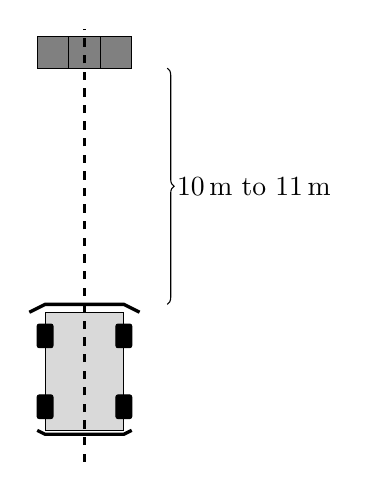
\begin{tikzpicture}
            \gokart{0}{0}{0}
        
            %Wall (three cubes)
            \draw[fill=gray] (-0.6,3) rectangle (-0.2,3.4);
            \draw[fill=gray] (-0.2,3) rectangle (0.2,3.4);
            \draw[fill=gray] (0.2,3) rectangle (0.6,3.4);
        
            %Dashed line from go-kart to wall
            \draw[dashed, thick] (0,-2) -- (0,3.5);

            \draw [decorate, decoration = {brace, raise=10pt}] (0.7,3) -- (0.7, 0) node[pos=0.5,right=10pt,black]{\SIrange{10}{11}{\meter}};
        \end{tikzpicture}
    %}
    \caption{Test scenario}
    \label{fig:test_scenario}
\end{figure}
The experimental setup consists of a Texas Instruments IWR6843AOPEVM development board, featuring the IWR6843AOP mmWave radar sensor, mounted at the front of a vehicle.  
The sensor provides point cloud data enriched with range, angle, and Doppler velocity information.  
This data forms the basis for the processing pipeline and enables the evaluation of radar odometry performance under realistic driving scenarios.  


\subsection{Sub-Tasks}

The research objective, together with the constraints of using a single radar sensor, implied several practical sub-tasks:  
\begin{itemize}
    \item Designing a pipeline to acquire and decode raw radar data.  
    \item Investigating suitable sensor configurations to balance field of view, update rate, and data density.  
    \item Implementing clustering methods to structure radar detections and isolate relevant features.  
    \item Integrating Doppler velocity information into the odometry estimation process.  
    \item Developing scan-to-scan registration using iterative closest point (ICP) optimization.  
    \item Employing submap aggregation to mitigate sparsity and improve stability.  
    \item Incorporating cluster-based tracking to filter dynamic objects from the ego-motion estimation.  
    \item Validating the complete system using recorded datasets and controlled driving experiments.  
\end{itemize}

As each sub-task builds upon the results of the previous one, the work followed an iterative and modular development approach, enabling gradual integration and continuous evaluation of the proposed system.  
\newpage

\section{IWR6843 Radar Interface and Configuration}
\label{sec:IWR6843 Radar Interface and Configuration}
The IWR6843AOPEVM development board from Texas Instruments features the IWR6843AOP, a high performance 4D mmWave FMCW radar sensor with Antenna On Package (AOP) design.
Although IWR6843AOP is intended for industrial applications and its complementary chip, AWR6843AOP, for automotive applications, IWR6843AOP was used in this project because it is available in the form of this development board and the two chips are identical in terms of their functionalities, only differing in compliance with automotive  industry \cite{iwr_awr_diff}.
Its small physical size, due to its AOP design, makes it an optimal choice for the desired mounting position, the go-kart's steering column.
\begin{figure}[!htbp]
    \centering
    \includegraphics[width=0.7\linewidth]{images/iwr6843aopevm-angled.png}
    \caption{IWR6843AOP sensor}
    \label{fig:IWR6843AOP sensor}
\end{figure}
\par
The IWR6843AOP radar sensor operates within the frequency range of \SIrange{60}{64}{\giga\hertz} and integrates 4 receive (RX) and 3 transmit (TX) antennas, radio frequency (RF) front-end stages, analog signal processing, and digital signal processing (DSP).
It offers a wide range of communication interfaces including SPI, I2C, CAN-FD, UART and LVDS for raw data access and an Arm Cortex-R4F microcontroller for user-applications \cite{dev_board_page}.
\begin{figure}[!htbp]
    \centering
    \includegraphics[width=1.0\linewidth]{images/blockdiagram.png}
    \caption{IWR6843AOP internal Block Diagram}
    \label{fig:IWR6843AOP_internal}
\end{figure}
\FloatBarrier\noindent
Texas Instruments offers various demo applications for the development board that utilize the internal microcontroller for showcasing the radar sensor's capabilities in different specialized scenarios.
It was found out that most of them only use the radar sensor itself only for obtaining a point cloud, which points include spatial information in form of $x,y,z$ coordinates and a radial speed information (the prior mentioned four dimensions of the sensor).
Application-specific processing of the point cloud itself is executed on an external computation device.
\par
The main demo application ("mmWave SDK demo") allows a versatile customization of the radar sensor's operating parameters and its discrimination capabilities while outputting the point cloud via its UART interface, accessible via the on-board USB to UART converter.
Although the demo seems to be intended to be used only for demonstration purposes, many projects based on Texas Instruments' mmWave radar sensors utilize it, because it poses a generic solution for obtaining (close to) real-time point cloud data from the sensor without prior development of a custom user-application for the radar sensor's internal microcontroller.
This setup was therefore chosen for supplying the emergency braking system with data.

\subsection{Utilizing the mmWave SDK demo}
The "mmWave SDK demo" was developed by Texas Instruments for showcasing the abilities of their mmWave radar sensors.
It consists of the radar sensor itself, supplying close to real-time point cloud data and an online tool for visualization of the raw output data and for the creation of a sequence of commands used for configuration of the radar sensor's operating parameters and output \cite{mmwave_demo_doc}.
Due to the demo's simple structure and the radar sensor's generic output, the online application can be replaced by a custom application replicating the online tool's behavior for making use of the data.
\par
In the demo application, the radar sensor opens two UART connections.
One connection is bidirectional at a lower speed of \SI{115200}{\baud} which is used to configure the radar sensor by sending the previously mentioned sequence of commands. 
The second connection is unidirectional, from the radar sensor to the receiver, at a higher speed of \SI{921600}{\baud} and is used for outputting a constant data stream after the radar sensor received its configuration and a start command.
As the data packets are encoded in a proprietary format and therefore need to be parsed prior to further processing, a custom software module was written in C++ and later ported to Python.
The module handles the radar sensor's setup by sending a configuration file containing the sequence of initialization commands and the cyclic parsing of the encoded data packets.
The sequence of commands was generated with Texas Instruments' online tool, as it provided graphical feedback while making the necessary compromises involved in setting up the radar sensor's operating parameters.

\subsection{Sensor Data Output Format}
As the data packets, containing the individual frames, are encoded in a proprietary format, they need to be parsed to allow for further processing.
Each frame starts with a frame header and contains a number of TLVs (Type, Length, Value) in which the actual payload data is stored\cite{mmwave_demo_doc}.
\begin{figure}[!htbp]
    \centering
    \includegraphics[width=0.4\linewidth]{images/UARTFrame.png}
    \caption{Frame structure. From \cite{mmwave_demo_output}.}
    \label{fig:UART data output format}
\end{figure}
\FloatBarrier\noindent
The frame's header has a total length of \SI{40}{\byte} and starts with a fixed magic word that denotes the start of each frame.
It also provides several other information in addition to the total packet length in bytes which is used to find the frame's end:
\begin{itemize}
    \item Magic Word: This value indicates the start of a new header, meaning that it can be used as a starting point for processing each frame.
    \item Total Packet Length: Total number of bytes in the frame (including the header) which can be used to calculate the frame's end.
    \item Platform: Indicates the device type and can be used for validating the radar sensor type. In the case of the device used for this project (IWR6843AOP) the expected value is "$0xA6843$".
    \item Number of TLVs: Total number of TLV's that exist in that specific frame.
\end{itemize}
\begin{figure}[!htbp]
    \centering
    \includegraphics[width=1.0\linewidth]{images/FrameFormatHeader.png}
    \caption{Frame header format. From \cite{mmwave_demo_output}.}
    \label{fig:Frame header format}
\end{figure}
\FloatBarrier\noindent
The frame contains one or more TLVs after its header.
Each TLV has a header itself in which it specifies its length and which type of data (point cloud, doppler heatmaps, statistics, ...) is contained inside.
Each TLV type needs to be decoded differently, as it represents a different type of data.
\begin{figure}[!htbp]
    \centering
    \includegraphics[width=0.95\linewidth]{images/TLVHeader.png}
    \caption{TLV header format. From \cite{mmwave_demo_output}.}
    \label{fig:TLV header format}
\end{figure}
\FloatBarrier

\subsection{Sensor Tuning}
As some operating parameters influence each other, their selection must be done carefully while observing the influence of the trade-offs involved.
This could be referred to as "sensor tuning" and is a critical step because it directly impacts the system's accuracy and performance.
\begin{comment}
Proper sensor tuning is critical because it directly impacts the accuracy and performance of the self-speed estimation, including the precision of the radial velocity and distance measurements derived from the returned radar waves.

Before initiating the sensor setup, it is crucial to identify the key parameters that will be monitored and adjusted. These parameters determine which aspects of the sensor's configuration need modification and help define the target performance criteria. Examples of these parameters include:
\end{comment}
The following operating parameters can be tuned:
\begin{itemize}
    \item Frame rate
    \item Range resolution
    \item Maximum unambigious range
    \item Maximum radial velocity
    \item Radial velocity resolution
\end{itemize}

Tuning these operating parameters introduces trade-offs by influencing each other in the following ways:
\begin{table}[h]
    \centering
    \resizebox{\columnwidth}{!}{%
    \begin{tabular}{|l|l|p{3.5cm}|p{3.5cm}|p{3.5cm}|}
        \hline
        \textbf{Tuning Parameter} & \textbf{Effect on Performance} & \textbf{Related HW Block} & \textbf{Trade-Off} \\
        \hline
        Frame Rate & Higher FPS = faster updates but more processing load & C674x DSP, Radar Data Memory & Higher FPS reduces maximum range \\
        \hline
        Range Resolution & Higher resolution = better object separation & ADC, 1D FFT (Range FFT) & Higher resolution reduces max range \\
        \hline
        Maximum Range & Determines farthest detectable object & RF Front-End, PA, LNA, ADC & Higher range lowers resolution \\
        \hline
        Radial Velocity Resolution & Improves speed accuracy & DSP, 2D FFT (Doppler FFT) & Higher resolution requires more chirps \\
        \hline
        Maximum Radial Velocity & Detects fast-moving objects & Chirp rate, TX Antennas, 2D FFT & Higher max velocity reduces resolution \\
        \hline
        %% [24/03/2025] Leander: Commented out because RCS depends on the target can not be tuned; is only used as a reference for calculating the range and stuff like this
        %Radar Cross Section (RCS) & Controls detection sensitivity based on object reflectivity & RF Front-End, LNA, ADC, DSP Filtering & Higher RCS increases range but may include unwanted reflections; Lower RCS improves accuracy but may miss small objects \\
        %\hline
    \end{tabular}%
    }
    \caption{Radar System Tuning Parameters and Trade-offs}
    \label{tab:mmWave_Sensor_Parameters}
\end{table}
The resulting overall accuracy of the velocity and distance measurements is again dependent on these operating parameters:
\begin{itemize}
    \item Radial velocity accuracy: A fine balance between velocity resolution and frame rate must be maintained to ensure precise doppler shift measurements. Lower resolution results in rounded velocity values, while an excessively high frame rate may introduce computational bottlenecks.
    \item Distance accuracy: Optimizing range resolution and maximum range ensures that detected objects are positioned accurately within the environment. Increasing range often sacrifices resolution, leading to potential inaccuracies in close-range detections.
    \item Signal Processing Considerations: The FFT calculation parameters directly affect both range and doppler calculations, influencing the ability to distinguish between objects and detect small velocity variations.
\end{itemize}
This shows that finding exact values for the operation parameters by adjusting them while carefully watching their influences is crucial and heavily dependent on the particular application.
The test scenario required an unambigious range of at least \SI{10}{\meter} and a maximum radial velocity of \SI{10}{\meter\per\second} due to its boundary conditions, together with the desire of the highest possible resolution of the radial velocity to ensure a reliable operation of the radar-based self-speed estimation.
Tuning yieled a configuration with the following operating parameters:
\begin{itemize}
    \item Frame rate: \SI{30}{\frame\per\second}
    \item Range resolution: \SI{0.178}{\meter}
    \item Maximum unambigious range: \SI{18.22}{\meter}
    \item Maximum radial velocity: \SI{10.24}{\meter\per\second}
    \item Radial velocity resolution: \SI{0.16}{\meter\per\second}
\end{itemize}

Tuning and choosing the sensor's parameters carefully is extremely important as it defines the accuracy of 
therefore influences the reliability of the entire radar system.
Fine-tuning these settings ensures that the sensor operates optimally, enabling more precise self-speed estimation and overall system performance.
The accuracy of radial speed estimation and distance measurements depends directly on the tuning of these parameters. A poorly configured sensor can result in erroneous velocity estimations, unreliable object detection, or excessive noise in Doppler measurements. An example of the influence of the selection of the correct parameters on the output point cloud of the radar sensor can be found in Fig.~\ref{fig:IWR6843AOP Calibration example2 for the sensor}.

\begin{figure}[!htbp]
    \centering
    \includegraphics[width=1.0\linewidth]{images/calib_ex.png}
    \caption{Output of the IWR6843AOP prior sensor tuning.}
    \label{fig:IWR6843AOP Calibration example for the sensor}
\end{figure}

\begin{figure}[!htbp]
    \centering
    \includegraphics[width=1.0\linewidth]{images/calib_ex2.png}
    \caption{Output of the IWR6843AOP after sensor tuning.}
    \label{fig:IWR6843AOP Calibration example2 for the sensor}
\end{figure}

\FloatBarrier
\section{CHIRP Sequence Configuration}

\label{sec:chirp-theory}

To enable effective ego-motion estimation, the radar must be configured with a suitable chirp profile that balances range and velocity resolution.
This is achieved through the configuration of Frequency-Modulated Continuous Wave (FMCW) chirps, which define how the radar sweeps frequencies over time to capture environmental information.

In millimeter-wave FMCW radar systems such as the IWR6843, a chirp refers to a signal whose frequency increases (or decreases) linearly over a defined bandwidth $B$ during a fixed duration $T_c$.
When this signal reflects off a target and returns to the radar, the delay between transmitted and received signals encodes range information.
The Doppler shift between multiple received chirps in a frame encodes relative velocity.  
As seen in Figure~\ref{fig:radarWavePropagation}, the reflected wave varies in phase and frequency depending on object motion.


\begin{figure}[!htbp]
    \centering
    \includegraphics[width=0.5\linewidth]{images/radarWave.png}
    \caption{Radar 60-64GHz radio wave reflection.}
    \label{fig:radarWavePropagation}
\end{figure}

Each chirp is defined by the following core parameters:
\begin{itemize}
    \item Start frequency $f_0$
    \item Frequency slope $S$
    \item Chirp duration $T_c$
    \item Idle time between chirps $T_{idle}$
    \item Sampling rate $f_s$
    \item Bandwidth $B = S \cdot T_c$
\end{itemize}

\hfill

From these parameters, the radar sensing capabilities are derived as follows:

\begin{itemize}
    \item \textbf{Range resolution:} 
    \[
        \Delta R = \frac{c}{2B}
    \]
    where $c$ is the speed of light and $B$ is the chirp bandwidth.

    \item \textbf{Maximum unambiguous range:} 
    \[
        R_{max} = \frac{c f_s}{2S}
    \]
    where $f_s$ is the ADC sampling rate and $S$ is the frequency slope.

    \item \textbf{Velocity resolution:} 
    \[
        \Delta v = \frac{\lambda}{2 N_c T_c}
    \]
    where $\lambda$ is the wavelength, $N_c$ is the number of chirps per frame, and $T_c$ is the chirp duration.

    \item \textbf{Maximum unambiguous velocity:} 
    \[
        v_{max} = \frac{\lambda}{4 T_c}
    \]
    assuming uniform chirp spacing.
\end{itemize}

These equations clearly show that both range and velocity resolution depend directly on the chirp design.

\vspace{1em}
\newpage

\subsection{Chirp Design Strategies and Trade-offs}
\label{sec:chirp-strategies}

Radar applications differ in their emphasis on range vs velocity accuracy.
Odometry requires both.
We now examine key chirp configuration strategies and discuss their trade-offs.
\vspace{1em}

\subsubsection*{(1) Full-Bandwidth Chirp (Single 4~GHz Sweep)}

A single chirp sweeping across the entire 4~GHz available bandwidth provides the finest possible range resolution.
This is ideal for tasks requiring precise spatial localization of static objects.

\textbf{Trade-offs:}
\begin{itemize}
    \item \textbf{Pros:} Excellent range resolution ($\Delta R$ minimized).
    \item \textbf{Cons:} High ADC sampling rates required. Limits maximum measurable range ($R_{max}$). Increases noise sensitivity. Not ideal for multi-radar systems due to potential mutual interference.
\end{itemize}

\begin{figure}[!htbp]
    \centering
    \includegraphics[width=1.0\linewidth]{images/profile_full_4GHz.png}
    \caption{Single 4~GHz chirp.}
    \label{fig:profile4GHz}
\end{figure}

{\small
\textit{Conclusion:} Best for high-resolution mapping in single-device systems.
May suffer in multi-radar setups due to wide spectral overlap.
}

\vspace{1em}

\subsubsection*{(2) Divided-Band Chirps (Multiple Shorter Sweeps)}

An alternative is to split the full 4~GHz bandwidth into multiple chirps with reduced individual sweep widths (e.g., 2~GHz).
Each chirp provides moderate resolution.

\textbf{Trade-offs:}
\begin{itemize}
    \item \textbf{Pros:} Reduced ADC load. Allows frequency diversity across chirps.
    \item \textbf{Cons:} Each individual chirp has worse $\Delta R$ than full sweep. However, averaging multiple bands improves robustness.
\end{itemize}

\begin{figure}[!htbp]
    \centering
    \includegraphics[width=1.0\linewidth]{images/profile_two_2GHz.png}
    \caption{Two 2~GHz chirps in the same frame.}
    \label{fig:profile2GHz}
\end{figure}

{\small
\textit{Conclusion:} Balanced design.
Useful in scenarios requiring robustness against channel noise or radar interference.
Also reduces overlap when multiple radars are active.
}

\vspace{1em}

\subsubsection*{(3) Mixed Chirp Strategy (Full-Band + Narrow-Band Chirps)}

Combining different chirp types in a single frame can provide both high range and velocity resolution.
For example, use one full-band chirp for precise range, followed by multiple narrow-band chirps for velocity estimation.

\textbf{Trade-offs:}
\begin{itemize}
    \item \textbf{Pros:} Leverages benefits of both strategies. Improves multi-parameter resolution without overwhelming hardware.
    \item \textbf{Cons:} Increases configuration complexity. Requires advanced processing and careful interleaving.
\end{itemize}

\begin{figure}[!htbp]
    \centering
    \includegraphics[width=1.0\linewidth]{images/profile_full_4GHz_2GHz.png}
    \caption{Overlay of single 4~GHz chirp and two 2~GHz chirps.}
    \label{fig:profile2And4GHz}
\end{figure}

{\small
\textit{Conclusion:} Best suited for ego-motion and odometry applications.
Can support multi-device environments with careful planning.
}

\begin{table}[h]
    \centering
    \caption{Comparison of Chirp Configuration Strategies}
    \label{tab:chirp_comparison}
    \resizebox{\columnwidth}{!}{%
    \begin{tabular}{|p{3.5cm}|p{3.2cm}|p{3.5cm}|p{3.8cm}|}
        \hline
        \textbf{Chirp Strategy} & \textbf{Range Resolution} & \textbf{Velocity Resolution} & \textbf{Best Use Case} \\
        \hline
        Full-Bandwidth Chirp (4 GHz) &
        High (Fine $\Delta R$) &
        Moderate (Few chirps/frame) &
        Precise mapping in single-radar setups; spatial accuracy prioritized \\
        \hline
        Divided-Band Chirps (e.g., 2×2 GHz) &
        Moderate (per chirp), improved via averaging &
        Moderate to High (more chirps/frame possible) &
        Robust odometry in noisy or multi-radar environments \\
        \hline
        Mixed Chirp Strategy (Full + Narrow) &
        High (from full chirp), plus enhanced Doppler &
        High (from multiple narrow chirps) &
        Ego-motion estimation; combines benefits of both range and Doppler precision \\
        \hline
    \end{tabular}%
    }
\end{table}

\vspace{1em}

The table above summarizes the key performance characteristics and use cases for each chirp configuration strategy.

The Full-Bandwidth Chirp maximizes spatial resolution, making it ideal for scenarios where high-fidelity mapping of nearby static objects is required—such as indoor SLAM or obstacle-rich environments. 
However, its wide spectral footprint and high ADC demand make it less suitable in systems where multiple radar devices operate simultaneously, as mutual interference becomes likely.
The Divided-Band Chirp approach offers a middle ground.
By allocating portions of the spectrum to separate chirps, it reduces system load and provides flexibility in processing. 
While individual chirps have lower range resolution, combining information across them improves detection stability. This strategy excels in distributed radar systems, such as in collaborative or multi-node sensor networks, where frequency coordination helps reduce ghost targets and interference.
Finally, the Mixed Chirp Strategy integrates the strengths of both previous approaches. 
A full-band chirp ensures accurate spatial anchoring, while narrow-band chirps provide temporal and Doppler refinement. 
This makes it the most adaptive option for applications like ego-motion estimation, where both precise localization and motion cues are critical. 
Its complexity, however, demands a more advanced signal processing pipeline and careful calibration to ensure synchronization between chirps.

In multi-radar environments, especially in close proximity (e.g., autonomous fleets or dual-radar vehicles), selecting chirp strategies that reduce spectral overlap is essential. Techniques like time-division multiplexing, slope diversity, and chirp staggering become critical tools to mitigate false detections and interference.

\vspace{1em}

\subsection{Chirp Configuration for Multi-Radar Systems}
\label{sec:chirp-multiradar}

When deploying multiple radar devices (e.g., front-left, front-right), interference becomes a significant challenge.
Simultaneous transmission using overlapping chirp frequencies can lead to ghost detections, false targets, and degraded signal-to-noise ratio. 
This due to the radio waves that are transmitter can cause collitions between each other creating this "ghost detections".
There are some strategies that can be employed to avoid this phenomenom.

\textbf{Recommended strategies:}
\begin{itemize}
    \item Use \textbf{non-overlapping frequency ranges} per device (e.g., 60–62~GHz on left, 62–64~GHz on right).
    \item Apply \textbf{interleaved chirps} in time: stagger chirps across sensors.
    \item Utilize \textbf{different slope values}: reduces likelihood of constructive interference.
    \item Match chirp \textbf{idle times} to ensure orthogonality.
\end{itemize}

These methods are essential to avoid ghost detections and preserve spatial coherence across sensors.

\vspace{1em}

{\small
\textit{Conclusion:} Chirp configuration in multi-radar environments requires trade-offs between resolution and isolation.  
Design must ensure orthogonality to avoid mutual interference.
}

\vspace{1em}

\subsection{Summary}

The configuration of chirps in FMCW radar defines its core capabilities in range and velocity estimation.
Depending on the target application — whether precision mapping, ego-motion tracking, or multi-device deployment — the choice of chirp bandwidth, duration, slope, and sequencing must be carefully made.

The following considerations are essential:
\begin{itemize}
    \item Use wide-band chirps when range precision is critical.
    \item Use many chirps with long frame durations when velocity resolution is prioritized.
    \item Use divided-band or mixed strategies in multi-radar systems to balance robustness and prevent interference.
\end{itemize}

Careful design enables robust radar odometry, reliable environment mapping, and scalable multi-radar systems.


\section{Pipeline Implementation: Modules Implemented and Mathematical Explanation}
\label{sec:Mathematical Models and Algorithms for Radar-Based Object Detection}

To reliably interpret radar sensor data for static object detection and ego-motion estimation, a modular processing pipeline was developed. 
This pipeline supports both single-radar and dual-radar configurations, in both cases the inclusion of an Inertial Measurement Unit (IMU) is needed to compensate for rotational motion of the platform. 
The modular design allows adaptation to different vehicle setups and deployment conditions.

\subsection*{Sensor Data Preprocessing}
In the preprocessing of the radar data, there are two scenarios that were implemented for this project, the single-radar setup and the dual-radar setup with IMU integration.
In both radar setups, radar data is received over UART in the form of raw frames containing point cloud information. 
Each point includes its spatial coordinates $(x, y, z)$, radial velocity $v_r$, side-point info; this information comes with signal-to-noise ratio (SNR) and noise ration (dB) values that indicate the quality of each detection and range profile data.

The raw bytes are decoded \cite{understanding_uart} and structured into frame objects, which are then passed through a Physical Transformation module. 
This step converts from the sensor frame coordinates into the vehicle local frame, accounting for radar mounting position and orientation. 
This can be consider a rigid body transformation involving rotation and translation matrices.
However is really important that this process of rigid transformation is done, as the data that we obtain from the sensor does not know where it is in the vehicle, creating a missalignment between the radar data and the vehicle frame of reference.

\subsubsection*{Dual-Radar Configuration}
In the dual-radar configuration, two front-facing sensors are mounted symmetrically on the left and right sides of the vehicle, providing overlapping fields of view. 
This arrangement expands the effective coverage and reduces blind spots, offering a broader perception range compared to a single-radar setup.  

The use of two radars requires careful calibration to avoid interference effects, such as ghost detections or false targets, and to ensure consistent alignment of their outputs.  
When properly tuned, the dual-radar configuration produces a denser and more reliable point cloud, serving as a stronger foundation for subsequent stages of the odometry pipeline.

\subsection*{Frame Aggregation}
Radar point clouds are naturally sparse, especially at longer ranges. 
To improve stability and robustness, consecutive frames are aggregated into a local submap. 
This approach increases point density, reduces the effect of random noise, and provides a richer structure for downstream tasks such as clustering and alignment. 
The aggregation is performed after IMU-based alignment, ensuring that the fused frames are geometrically consistent. 

\subsection*{Filtering and Self-Speed Estimation}
Once points are aggregated and aligned, the pipeline performs filtering in two stages:

\begin{itemize}
    \item \textbf{Coordinate and SNR Filtering:} Removes points outside valid spatial boundaries or below a configurable SNR threshold.
    \item \textbf{Velocity-based Filtering:} Applies a Doppler threshold to remove points with radial velocities below or above predefined limits. This eliminates static clutter and extreme outliers, leaving only detections within the valid motion range.
\end{itemize}

From the remaining points, the vehicle self-speed is estimated using the Doppler measurements. 
A Kalman filter is then applied to smooth fluctuations and provide a stable velocity estimate, which is reused in subsequent stages of the odometry pipeline.

\subsection*{Clustering and Outlier Rejection}
The filtered detections are organized into clusters to provide structure to the radar scene. 
A two-stage clustering strategy is employed to gradually refine the set of candidate targets:  

\begin{itemize}
    \item \textbf{Stage 1 – Permissive Clustering:} A loose grouping is applied using the DBSCAN algorithm, which is well-suited for radar point clouds since it does not require the number of clusters to be specified in advance and can naturally separate sparse detections. 
    At this stage, the parameters are set permissively, allowing loosely associated points to be grouped into preliminary clusters so that potential targets are not discarded prematurely.  
    \item \textbf{Stage 2 – Strict Clustering:} The preliminary clusters are reprocessed with stricter DBSCAN parameters, enforcing tighter geometric proximity between points. 
    This refinement step eliminates loosely connected points and isolates only the detections that are spatially consistent, resulting in compact and reliable target clusters.  
\end{itemize}

This hierarchical approach ensures that targets are first captured broadly and then refined to retain only geometrically close detections, which are more suitable for downstream odometry estimation.  
Additionally, RANSAC-based outlier rejection is performed prior to clustering, further reducing the influence of inconsistent or spurious points on the cluster formation.  

DBSCAN's ability to handle varying cluster shapes, adapt to density variations, and explicitly label noise points makes it particularly advantageous in radar applications, where detections are inherently sparse, noisy, and often non-uniformly distributed.

\subsection*{ICP Alignment and Ego-Motion Estimation}
The final stage of the pipeline estimates vehicle motion by applying the Iterative Closest Point (ICP) algorithm for frame-to-frame alignment. 
ICP iteratively minimizes the distance between corresponding points across consecutive frames, computing the rigid-body transformation that best aligns them.  

In this project, ICP was applied under two distinct configurations for analysis:  

\begin{itemize}
    \item \textbf{Global ICP:} The entire aggregated point cloud from consecutive frames is used for alignment. 
    This approach provides a direct estimate of ego-motion but is sensitive to outliers and dynamic objects present in the scene.  

    \item \textbf{Cluster-based ICP:} Instead of aligning full point clouds, ICP is applied selectively on clusters identified as static targets. 
    By focusing on geometrically consistent regions, this method looks to improve robustness against moving objects and to enhance the stability of the motion estimate.  
\end{itemize}

The outcome of ICP is a rigid transformation that represents the vehicle's ego-motion between frames, serving as the foundation for radar-based odometry.

\begin{figure*}[!htbp]
    \centering
    \resizebox{\textwidth}{!}{%
        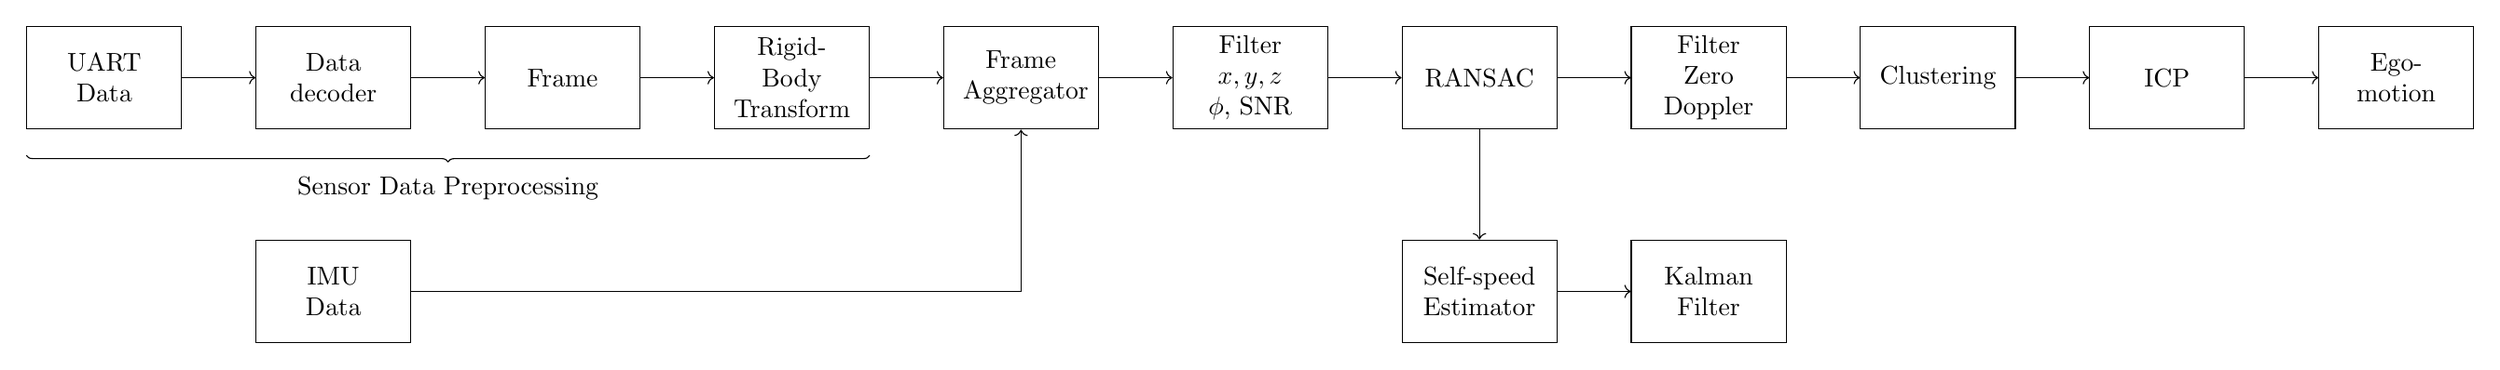
\begin{tikzpicture}
            % Block style
            \tikzstyle{block} = [rectangle, draw, text width=4.5em, text centered, minimum width=6em, minimum height=4em]

            % Upper row
            \node[block] (uart) {UART\\Data};
            \node[block, right=of uart] (decoder) {Data decoder};
            \node[block, right=of decoder] (frames) {Frame};
            \node[block, right=of frames] (transform) {Rigid-Body\\Transform};
            \node[block, right=of transform] (frame_aggr) {Frame\\Aggregator};
            \node[block, right=of frame_aggr] (coord_filter) {Filter\\$x,y,z$\\$\phi$, SNR};
            \node[block, right=of coord_filter] (ransac) {RANSAC};
            \node[block, right=of ransac] (doppler_filter) {Filter\\Zero Doppler};
            \node[block, right=of doppler_filter] (clustering) {Clustering};
            \node[block, right=of clustering] (icp) {ICP};
            \node[block, right=of icp] (ego) {Ego-motion};

            % IMU and self-speed estimator (below RANSAC)
            \node[block, below=1.5cm of decoder] (imu) {IMU\\Data};
            \node[block, below=1.5cm of ransac] (self_speed_estim) {Self-speed Estimator};
            \node[block, right=of self_speed_estim] (self_speed_kalman) {Kalman Filter};

            % Connections
            \draw[->] (uart) -- (decoder);
            \draw[->] (decoder) -- (frames);
            \draw[->] (frames) -- (transform);
            \draw[->] (transform) -- (frame_aggr);
            \draw[->] (imu.east) -| ([yshift=-1.5em]frame_aggr.south) -| (frame_aggr.south);

            \draw[->] (frame_aggr) -- (coord_filter);
            \draw[->] (coord_filter) -- (ransac);
            \draw[->] (ransac) -- (doppler_filter);
            \draw[->] (doppler_filter) -- (clustering);
            \draw[->] (clustering) -- (icp);
            \draw[->] (icp) -- (ego);

            \draw[->] (ransac.south) -- (self_speed_estim.north);
            \draw[->] (self_speed_estim) -- (self_speed_kalman);

            % Bottom brace for preprocessing
            \draw [decorate, decoration = {brace, mirror, raise=10pt}]
                (uart.south west) -- (transform.south east)
                node[pos=0.5,below=15pt,black]{Sensor Data Preprocessing};
        \end{tikzpicture}
    }
    \caption{Single Radar Pipeline}
    \label{fig:single_radar_pipeline}
\end{figure*}

\begin{figure*}[!htbp]
    \centering
    \resizebox{\textwidth}{!}{%
        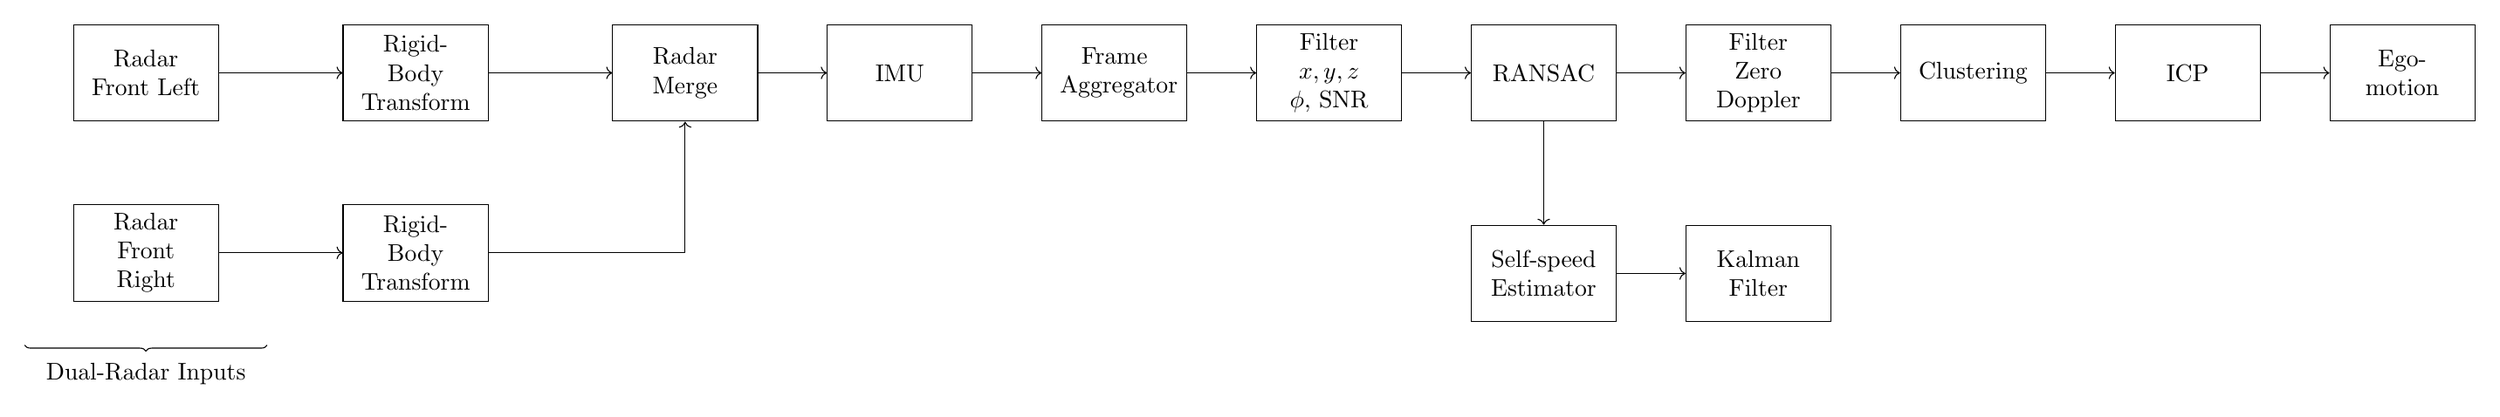
\begin{tikzpicture}
            % Block style
            \tikzstyle{block} = [rectangle, draw, text width=4.5em, text centered, minimum width=6em, minimum height=4em]

            % Input branches
            \node[block] (radar1) {Radar\\Front Left};
            \node[block, below=1.2cm of radar1] (radar2) {Radar\\Front Right};

            % Physical transformation
            \node[block, right=1.8cm of radar1] (transform1) {Rigid-Body\\Transform};
            \node[block, below=1.2cm of transform1] (transform2) {Rigid-Body\\Transform};

            % Merge and processing
            \node[block, right=1.8cm of transform1] (merge) {Radar Merge};
            \node[block, right=of merge] (imu) {IMU};
            \node[block, right=of imu] (frame_aggr) {Frame\\Aggregator};
            \node[block, right=of frame_aggr] (coord_filter) {Filter\\$x,y,z$\\$\phi$, SNR};
            \node[block, right=of coord_filter] (ransac) {RANSAC};
            \node[block, right=of ransac] (doppler_filter) {Filter\\Zero Doppler};
            \node[block, right=of doppler_filter] (clustering) {Clustering};
            \node[block, right=of clustering] (icp) {ICP};
            \node[block, right=of icp] (ego) {Ego-motion};

            % Self-speed estimator (below RANSAC)
            \node[block, below=1.5cm of ransac] (self_speed_estim) {Self-speed Estimator};
            \node[block, right=of self_speed_estim] (self_speed_kalman) {Kalman Filter};

            % Connections
            \draw[->] (radar1) -- (transform1);
            \draw[->] (radar2) -- (transform2);
            \draw[->] (transform1) -- (merge);
            \draw[->] (transform2) -| (merge);
            \draw[->] (merge) -- (imu);
            \draw[->] (imu) -- (frame_aggr);
            \draw[->] (frame_aggr) -- (coord_filter);
            \draw[->] (coord_filter) -- (ransac);
            \draw[->] (ransac) -- (doppler_filter);
            \draw[->] (doppler_filter) -- (clustering);
            \draw[->] (clustering) -- (icp);
            \draw[->] (icp) -- (ego);

            \draw[->] (ransac.south) -- (self_speed_estim.north);
            \draw[->] (self_speed_estim) -- (self_speed_kalman);

            % Bottom brace under radar2
            \draw [decorate, decoration = {brace, mirror, raise=8pt}] 
                ([xshift=-2em,yshift=-1em]radar2.south west) -- 
                ([xshift=2em,yshift=-1em]radar2.south east)
                node[midway, below=12pt] {Dual-Radar Inputs};
        \end{tikzpicture}
    }
    \caption{Dual Radar Pipeline}
    \label{fig:dual_radar_pipeline}
\end{figure*}



\FloatBarrier\noindent
\subsection{Sensor Data Preprocessing}
\label{subsec:transformations}

Each radar sensor in the dual-radar configuration is physically mounted with a specific orientation and tilt relative to the vehicle's forward direction. 
To ensure a common frame of reference for all points, it is necessary to compensate for:

\begin{itemize}
    \item \textbf{Yaw rotation}: due to angled placement (±30$^\circ$) of the radar modules.
    \item \textbf{Pitch tilt}: due to upward mounting tilt (15$^\circ$), which must be compensated to recover horizontal geometry.
    \item \textbf{Sensor offset}: due to the physical separation of the radar sensors in the horizontal axis (X-axis).
\end{itemize}

A yaw rotation \( R_{\text{yaw}} \) was first implemented, followed by a pitch correction \( R_{\text{pitch}} \), and finally a translation vector \( \vec{t} \) was applied to account for the physical position of the sensors with respect to the vehicle's coordinate origin.

The full transformation can be expressed as:

\begin{equation}
T_{\text{veh}} = R_{\text{yaw}} \cdot R_{\text{pitch}} \cdot \vec{p}_{\text{radar}} + \vec{T}
\label{eq:radar_to_vehicle_transform}
\end{equation}

Where:
\begin{itemize}
    \item \( \vec{p}_{\text{radar}} \) is a radar point in sensor coordinates.
    \item \( R_{\text{yaw}} \) is a 2D rotation around the vertical axis.
    \item \( R_{\text{pitch}} \) corrects for the upward sensor tilt.
    \item \( \vec{T} \) is the translation vector.
\end{itemize}

\vspace{1em}

Let $(x, y, z)$ be the original point from the radar frame, with $x$ to the right, $y$ forward, and $z$ upward. 
The transformations applied are as follows:

\paragraph{Yaw Correction (Z-axis Rotation)}
The radar sensors are rotated relative to the vehicle frame:

\begin{itemize}
    \item Radar A (Left): Mounted at $+30^\circ$ yaw $\Rightarrow$ compensated with $-30^\circ$ rotation.
    \item Radar B (Right): Mounted at $-30^\circ$ yaw $\Rightarrow$ compensated with $+30^\circ$ rotation.
\end{itemize}

The 2D rotation in the XY-plane is defined as:
\[
\begin{bmatrix}
x' \\
y' \\
z'
\end{bmatrix}
=
\begin{bmatrix}
\cos(\theta) & -\sin(\theta) & 0 \\
\sin(\theta) & \cos(\theta) & 0 \\
0 & 0 & 1
\end{bmatrix}
\begin{bmatrix}
x \\
y \\
z
\end{bmatrix}
\]

where $\theta = \pm30^\circ$ depending on the sensor.

\begin{figure}[!htbp]
    \centering
    \includegraphics[width=0.8\linewidth]{images/SensorsRotation.png}
    \caption{Yaw rotation of sensors around the Z-axis (±30$^\circ$).}
    \label{fig:z_axis_rotation}
\end{figure}

\vspace{2em}

\paragraph{Pitch Compensation (X-axis Rotation)}
Since the radar sensors are tilted upward by $15^\circ$, a corrective rotation around the X-axis is applied to bring the points back to a horizontal perspective: 

\[
\begin{bmatrix}
x' \\ y' \\ z'
\end{bmatrix}
=
\begin{bmatrix}
1 & 0 & 0 \\
0 & \cos(\phi) & -\sin(\phi) \\
0 & \sin(\phi) & \cos(\phi)
\end{bmatrix}
\begin{bmatrix}
x \\ y \\ z
\end{bmatrix}
\]

where $\phi = -15^\circ$ (negative to reverse the upward tilt).

\begin{figure}[!htbp]
    \centering
    \includegraphics[width=0.8\linewidth]{images/TiltSensor.png}
    \caption{Pitch compensation for $15^\circ$ upward tilt.}
    \label{fig:x_axis_rotation}
\end{figure}

\vspace{2em}

\paragraph{X-Axis Offset Compensation}
After rotation, each sensor's point cloud was translated along the X-axis to align with the vehicle's center:
\begin{itemize}
    \item Radar A: $x \leftarrow x - 0.32$ meters
    \item Radar B: $x \leftarrow x - 0.28$ meters
\end{itemize}

This translation ensured both sensors were aligned in a common vehicle-centric frame.

\begin{figure}[!htbp]
    \centering
    \includegraphics[width=0.8\linewidth]{images/RotationSensor.png}
    \caption{Final extrinsic configuration combining yaw, pitch, and translation.}
    \label{fig:extrinsics}
\end{figure}

\vspace{2em}

\paragraph{Impact of Transformations}
The importance of these corrections becomes evident when comparing raw and transformed data when the system data is unified in a single data set. 
Without transformations, detections from the left and right radars appear misaligned, producing duplicated or inconsistent clusters. 
After applying yaw, pitch, and translation compensation, the fused point cloud exhibits coherent structures, with static landmarks consistently overlapping across sensors.

Figures~\ref{fig:dualSensorCalib_2mts}--\ref{fig:AFTERdualSensorCalibRANSAC_2mts} illustrate this process, showing raw point clouds, clustered representations, and RANSAC fits before and after calibration. 
This information is of a person standing at 2 meters away form the vehicle, the process was decided as it was easy to visualize and to validate what was detected.
The transformed data serves as a stable basis for subsequent steps in the odometry pipeline, such as ICP-based submap alignment.

\begin{figure}[!htbp]
    \centering
    \includegraphics[width=0.9\linewidth]{images/dualSensorCalib_2mts.png}
    \caption{Raw dual-sensor point cloud before geometric transformations.}
    \label{fig:dualSensorCalib_2mts}
\end{figure}

\begin{figure}[!htbp]
    \centering
    \includegraphics[width=0.9\linewidth]{images/dualSensorCalibCluster_2mts.png}
    \caption{Clustered detections from both radars before transformation.}
    \label{fig:dualSensorCalibCluster_2mts}
\end{figure}

\begin{figure}[!htbp]
    \centering
    \includegraphics[width=0.9\linewidth]{images/dualSensorCalibRANSAC_2mts.png}
    \caption{RANSAC fit on Doppler velocities before transformation.}
    \label{fig:dualSensorCalibRANSAC_2mts}
\end{figure}

\begin{figure}[!htbp]
    \centering
    \includegraphics[width=0.9\linewidth]{images/AFTERdualSensorCalib_2mts.png}
    \caption{Fused point cloud after geometric transformations.}
    \label{fig:AFTERdualSensorCalib_2mts}
\end{figure}

\begin{figure}[!htbp]
    \centering
    \includegraphics[width=0.9\linewidth]{images/AFTERdualSensorCalibCluster_2mts.png}
    \caption{Clustered detections after transformation, showing improved alignment.}
    \label{fig:AFTERdualSensorCalibCluster_2mts}
\end{figure}

\begin{figure}[!htbp]
    \centering
    \includegraphics[width=0.9\linewidth]{images/AFTERdualSensorCalibRANSAC_2mts.png}
    \caption{RANSAC fit on Doppler velocities after transformation.}
    \label{fig:AFTERdualSensorCalibRANSAC_2mts}
\end{figure}

\vspace{1em}

\paragraph{Summary of Extrinsics}
\begin{itemize}
    \item \textbf{Left radar:} yaw $+30^\circ$, pitch $-15^\circ$, translation $(-0.32, 0, 0)$.
    \item \textbf{Right radar:} yaw $-30^\circ$, pitch $-15^\circ$, translation $(-0.28, 0, 0)$.
\end{itemize}

This extrinsic calibration ensures that dual-radar data is expressed in a coherent vehicle-centric frame, which is critical for downstream modules such as clustering, odometry, and obstacle tracking.


\subsection{Frame Aggregator}
\label{sec:Frame Aggregator}
The decoded frames are passed into a frame aggregator stage as a first step, which utilizes data aggregation to reduce possible data sparsity of individual frames. 
Data aggregation involves combining multiple consecutive data sets to create a more comprehensive and reliable dataset for processing. This approach increases both useful information and noise, but ultimately enhances the quality of radar point clouds for object detection and tracking stability.
For point clouds from radar sensors, aggregating multiple frames enhances data consistency and density, improving the system’s ability to reconstruct objects and detect motion patterns.

\subsubsection{Single Frame}
Using radar point cloud data from a single frame has inherent limitations, which can lead to incomplete or misleading detections:
\begin{itemize}
    \item A single frame may not capture enough points, leading to failed detections or incomplete object reconstruction.
    \item Limited point data can cause objects to appear fragmented or indistinguishable from noise.
\end{itemize}

\begin{figure}[!htbp]
    \centering
    \includegraphics[width=0.5\linewidth]{images/singleframe.png}
    \caption{Single Frame visualization.}
    \label{fig: Single Frame visualization}
\end{figure}

Consequently, it is difficult to precisely rebuild or map complex objects due to the limited points in the point cloud and information contained in a single radar frame, which results in ambiguity and uneven detection performance.
This ambiguity can result in the erroneous detection of a large object or the merging of two different objects into one, as the clustering or detection algorithm may malfunction, not due to inherent flaws in the algorithm itself, but rather due to the inherent flaws in the data. This phenomenon occurs when two or more objects are in close proximity from each other, but can not be distinguished from each other because of the lack of points in a single frame.

To mitigate these issues, frame aggregation can be leveraged, an approach supported by the Law of Large Numbers (LLN). By accumulating multiple frames, the impact of random variations can be reduced, such as:
\begin{equation}
    \frac{\sigma^2}{N}
    \label{eq:variance_per_sample_size}
\end{equation}
This leads to a more statistically stable representation of objects; which means that the larger the sample is, the less effect the noise will have. Additionally, variance reduction helps to filter out erroneous detections while improving the reliability of motion estimation.

\subsubsection{Multiple Frames}
In contrast, the aggregation of multiple frames can significantly enhance object detection capabilities.
Using this technique the algorithm can be tricked, by making it believe that there is more information that it was actually obtained from the single frame. This comes with the drawback that there will be some older data inside the processed frame.
\begin{figure}[!htbp]
    \centering
    \includegraphics[width=0.5\linewidth]{images/multiframe.png}
    \caption{Frame Aggregation visualization.}
    \label{fig: Frame Aggregation visualization}
\end{figure}

This aggregation approach improves the accuracy of velocity and trajectory estimations, strengthens object identification's resilience against transient noise, and reduces problems related to sparse data.
It was implemented by using a stack with a fixed size, executing a "pop" operation prior to the insertion of the new frame at the stack's end.
The point cloud containing the points of all frames stored in the frame aggregator is then passed to the next stage.
\subsection{x,y,z,SNR Filter}
The point cloud's points are passed through a first static filtering stage to remove points caused by noise, clutter or targets outside of the area of interest before being used for further processing.
This static filtering stage consists of four different filters, filtering out points by different attributes:
\begin{enumerate}
    \item Filtering by $SNR$: All points with a $SNR$ lower than \SI{12}{\deci\bel} are filtered out to remove points with a low signal and those that might be caused by noise or clutter.
    \item Filtering by $z$ coordinate: All points below a $z$ value of \SI{0}{\meter} and above \SI{2}{\meter} are filtered out to remove points caused by the ground or the ceiling.
    \item Filtering by $y$ coordinate: All points below a $y$ value of \SI{0.3}{\meter} are filtered out to remove points created by the driver's feet.
    \item Filtering by $\phi$: All points with an azimuth bigger than \SI{85}{\degree} are filtered out to remove points that are outside the area of interest.
\end{enumerate}
\textit{Note: The origin of the points' coordinate system is the sensor itself, so a coordinate of $(\SI{0}{\meter},\SI{0}{\meter},\SI{0}{\meter})$ is essentially at the sensor's mounting position and therefore approx. \SI{0.3}{\meter} above the ground.}
\par
As the static filtering stage only keeps points which are relevant in terms of there spatial position and $SNR$ for the following stages, it effectively decreases the computation time of each frame and prevents the following stages from processing invalid data.
The filtered point cloud is then passed to the next stages, the self-speed estimator and the dynamic filtering stage.

\begin{figure}[!htbp]
\centering
\begin{subfigure}{0.24\textwidth}
  \centering
  \includegraphics[width=\textwidth]{images/No_filter.png}
  \caption{Input}
\end{subfigure}
\begin{subfigure}{0.24\textwidth}
  \centering
  \includegraphics[width=\textwidth]{images/filter.png}
  \caption{Output}
\end{subfigure}
\caption{Example visualization of the input and output when filtering by the value of the $z$ coordinate.}
\label{fig:static_filter_z_example}
\end{figure}
\FloatBarrier\noindent



\subsubsection*{Static vs Non-static objects}
In the detected data there will always be static or moving objects in the field of view, this is more prominent when the sensor is mounted in a moving frame.
In this case every thing is moving from the perspective of the sensor, so how does the differentiation happens to identify statis vs non-static objects, this is simple, by leveraging on the doppler effect concept.
Using the doppler effect and understanding it is crutial for this step, as it is what will allow the algorithm to focuse the processing only in the static targets that are detected.

In this case, making the assumption that the sensor is mounted in a vehicle that goes 2 meters per second. With this in consideration, the assumption that all static targets should have a radial speed similar to the 2 meters per second.
This speed cannot be the same as the angle of detection can affect, the accuracy that may be obtained through the chirp configuration, etc.
Multiple variables can be added into this "equation", but the assumption that the static targets measured radial speed is close to the vehicle speed we can know which target to keep and which target to discard with only this paramter.

However that leaves us with the problem of how to group such targets. At this point the RANSAC algorithm becomes useful, as it will do the grouping for us, by ussing the radial speed.

\section{RANSAC-Based Motion Filtering}

To differentiate static and dynamic objects in the radar point cloud, we use a RANSAC-based approach on the relationship between azimuth angle $\theta$ and radial Doppler velocity $v_d$.

\subsection*{Principle}
Under ideal conditions, static objects exhibit Doppler values consistent with the vehicle's own motion and orientation. 
These values follow a smooth curve when plotted against azimuth. 
Moving objects, however, deviate from this pattern.
RANSAC (Random Sample Consensus) is used to robustly fit a model to the expected Doppler pattern of static objects. 
Points that do not conform to the model are classified as dynamic.

\subsection*{Mathematical Model}

We assume a second-degree polynomial relationship:
\[
v_d = a\theta^2 + b\theta + c
\]

RANSAC fits this model by iteratively:
\begin{itemize}
    \item Sampling minimal subsets of the data,
    \item Fitting the polynomial,
    \item Identifying inliers whose residual error is below a threshold,
    \item Selecting the model with the highest consensus.
\end{itemize}

Let $\mathbf{X}$ be the input azimuth values and $\mathbf{y}$ the Doppler speeds:

\[
\mathbf{X} = \begin{bmatrix} \theta_1 \\ \theta_2 \\ \vdots \\ \theta_n \end{bmatrix}, \quad 
\mathbf{y} = \begin{bmatrix} v_{d1} \\ v_{d2} \\ \vdots \\ v_{dn} \end{bmatrix}
\]

RANSAC estimates polynomial coefficients $\mathbf{w} = [a, b, c]^T$ such that:

\[
\mathbf{y} \approx \Phi(\mathbf{X}) \cdot \mathbf{w}, \quad
\Phi(\mathbf{X}) = 
\begin{bmatrix}
\theta_1^2 & \theta_1 & 1 \\
\theta_2^2 & \theta_2 & 1 \\
\vdots & \vdots & \vdots \\
\theta_n^2 & \theta_n & 1 \\
\end{bmatrix}
\]

\subsection*{Use in Pipeline}

This filtering step occurs after point-wise filtering (e.g., Doppler and range cuts). It outputs:
\begin{itemize}
    \item \textbf{Inliers} – points likely to be static (used in clustering/ICP)
    \item \textbf{Outliers} – likely dynamic, excluded from ego-motion estimation
\end{itemize}

%TODO: Fix image, use one from project.
\begin{figure}[!htbp]
    \centering
    \includegraphics[width=1.0\linewidth]{images/RANSAC.png}
    \caption{RANSAC fit of Doppler vs. azimuth. Inliers = static (blue), Outliers = moving (red). This is simulated data to illustrate the concept.}
    \label{fig:ransac_static_dynamic}
\end{figure}

\subsection{Static vs Dynamic Objects: Role of Doppler}

In radar-based perception, identifying dynamic objects (e.g., vehicles, pedestrians) amidst a cluttered scene of static structures (e.g., walls, poles) is critical.
This task becomes more complex when the radar is mounted on a moving platform, such as a vehicle.
From the sensor's perspective, **all objects appear to move** due to its own motion. The key to resolving this ambiguity lies in leveraging the **Doppler effect**.
The Doppler effect describes how the observed frequency of a wave changes based on the relative motion between the source and the observer. For radar systems, this translates into measurable **radial velocity** values: the component of an object's velocity along the line of sight of the radar.
Assuming the vehicle is moving at a constant speed (e.g., 2 m/s), static targets—such as buildings or parked cars—should exhibit Doppler values that align with this ego-motion, adjusted by their detection angle (azimuth).
That is, a static object located directly ahead will have a Doppler value close to $+2$ m/s (if approaching), while an object at the side (90 azimuth) will have nearly 0 m/s radial velocity.
This expected Doppler pattern for static objects traces a smooth curve when plotted against azimuth. Deviations from this curve indicate potential dynamic objects with their own independent motion.
To robustly extract this pattern from noisy measurements, **RANSAC** is applied to fit a second-order polynomial to the Doppler vs. azimuth data. This model captures the expected distribution of static points.
Points that significantly deviate from this model are considered **dynamic** and excluded from ego-motion estimation steps.

\paragraph{Benefits of RANSAC-Based Filtering:}
\begin{itemize}
    \item Ignores noisy or misdetected points by considering consensus.
    \item Segregates the scene into static (inliers) and dynamic (outliers) segments.
    \item Improves the accuracy of clustering and motion estimation by focusing only on consistent, stationary targets.
\end{itemize}

The filtered result not only enables accurate **object tracking**, but also prevents false ego-motion estimates that could arise from moving targets dominating the point cloud.
\subsection{Self-speed Estimator}
\label{sec:self-speed_estimator}
The vehicle's self-speed plays a crucial role in distinguishing between stationary and moving objects, as it enables the removal of dynamic points in later stages of the pipeline. 
It therefore needs to be determined in a reliable way.
Traditional approaches usually utilize external sensors such as wheel encoders, Global Positioning System (GPS), or Inertia Measurement Units (IMUs).
In this project, a technique was developed that determines the vehicle's self-speed only by processing the point cloud's data.
An angle $\phi_{p}$ was defined between each individual point of the point cloud and the radar sensor's centerline:
\par
\begin{figure}[!htbp]
    \centering
    %\resizebox{0.48\textwidth}{!}{
        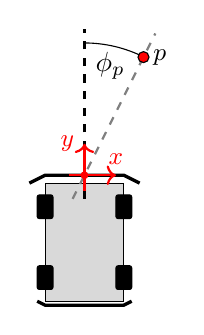
\begin{tikzpicture}
            \gokart{0}{0}{0}

            \coordinate(O) at (0,0);
            \coordinate(P) at (0.75,1.5);
            \coordinate(A) at (0,1.5);

            \draw[dashed, thick, gray] ($(P)!1.2!(O)$) -- ($(O)!1.2!(P)$);
            \draw[dashed, thick] ($(A)!1.2!(O)$) -- ($(O)!1.24!(A)$);
            \draw pic["$\phi_{p}$", draw=black, angle radius=1.68cm, angle eccentricity=0.85] {angle=P--O--A};
            \draw[fill=red] (P) circle (0.07) node [right] {\small $p$};

            \draw[->, thick, red] (-0.2,0) -- (0.4,0) node[above] {\small $x$};
            \draw[->, thick, red] (0,-0.2) -- (0,0.4) node[left] {\small $y$};
            \fill[red] (0,0) circle (0.05);
        \end{tikzpicture}
    %}
    \caption{Definition of the angle $\phi_{p}$}
    \label{fig:def_angle_phi}
\end{figure}
\FloatBarrier\noindent

\subsubsection*{Scalar Ego-Speed Estimation}
The first stage estimates the forward speed of the vehicle under the assumption of motion along the $+y$ axis. 
For each radar detection, the angle $\phi_p$ relative to the sensor's forward axis is defined (see Figure~\ref{fig:def_angle_phi}):  

\[
\phi_{p} = \arctan\left(\frac{x_p}{y_p}\right).
\]

The observed radial velocity of a static point $p$ depends on the vehicle speed $v_0$ and follows a cosine law:  

\[
v_{r,p}(v_0,\phi_p) = -v_0 \cdot \cos(\phi_p).
\]

Since no point lies exactly on $\phi=0^\circ$ and noise is present, all available inlier points (after RANSAC filtering) are used to fit a regression curve $v(\phi)$ to the measured pairs $(\phi_p, v_{r,p})$. 
The fitted value at $\phi = 0^\circ$ provides the best estimate of the scalar vehicle speed. 
A least-squares polynomial regression of order 2 is sufficient, since $\cos(\phi)$ can be locally approximated in the domain $\phi_p \in \left[-\frac{\pi}{2}, \frac{\pi}{2}\right]$ by:  

\[
\cos(\phi_p) \approx a \phi_p^2 + b.
\]

\subsubsection*{Generalized 2D Ego-Velocity Estimation}
The scalar approach assumes purely forward motion. 
To extend the model, the Doppler equation for a static point observed at angle $\theta$ is introduced:  

\[
v_{r}(\theta) = v_x \cos(\theta) + v_y \sin(\theta),
\]

where $v_x$ and $v_y$ are the ego-velocity components along the $x$ and $y$ axes of the vehicle frame.  
This equation is linear in $v_x$ and $v_y$, which allows solving for both components simultaneously using a least-squares approach across multiple points:  

\[
\begin{bmatrix}
v_{r,1} \\
v_{r,2} \\
\vdots \\
v_{r,n}
\end{bmatrix}
=
\begin{bmatrix}
\cos(\theta_1) & \sin(\theta_1) \\
\cos(\theta_2) & \sin(\theta_2) \\
\vdots & \vdots \\
\cos(\theta_n) & \sin(\theta_n)
\end{bmatrix}
\begin{bmatrix}
v_x \\ v_y
\end{bmatrix}.
\]

This formulation naturally integrates into the existing pipeline: RANSAC provides inlier points representing static structures, and the least-squares solution yields robust estimates of both forward and lateral velocity components.  

\subsubsection*{Practical Considerations}
Test runs demonstrated that the radar-only ego-velocity estimate closely followed the reference vehicle speed with a small static offset. 
However, fluctuations occurred in cases with sparse point clouds. 
This effect was mitigated by tuning the frame aggregation window and applying a Kalman filter after the regression stage, providing a stable and continuous self-speed estimate for downstream filtering and odometry estimation.  

\begin{figure}[!htbp]
    \centering
    \includegraphics[width=1.0\linewidth]{images/self_speed_reality.png}
    \caption{Example of radar-based self-speed estimation compared against the ground truth indicator.}
    \label{fig:self_speed_test_data}
\end{figure}

\FloatBarrier\noindent
The full process of ego-velocity estimation is summarized in Figure~\ref{fig:self_speed_block}. 
The radar point cloud is first filtered using RANSAC to retain only inliers corresponding to static structures. 
From these points, both the azimuth angle and Doppler velocity are extracted. 
At this stage, the pipeline branches into two estimation strategies:  

\begin{itemize}
    \item \textbf{Scalar ego-speed estimation:} a polynomial regression approximates the cosine law of Doppler velocities, yielding the forward velocity component only.
    \item \textbf{2D ego-velocity estimation:} a linear least-squares solution of the Doppler equation
    \[
    v_{r}(\theta) = v_x \cos(\theta) + v_y \sin(\theta)
    \]
    provides both longitudinal ($v_y$) and lateral ($v_x$) velocity components simultaneously.
\end{itemize}

Both outputs are subsequently passed through a Kalman filter for temporal smoothing before being used in the downstream pipeline.

\begin{figure}[!htbp]
    \centering
    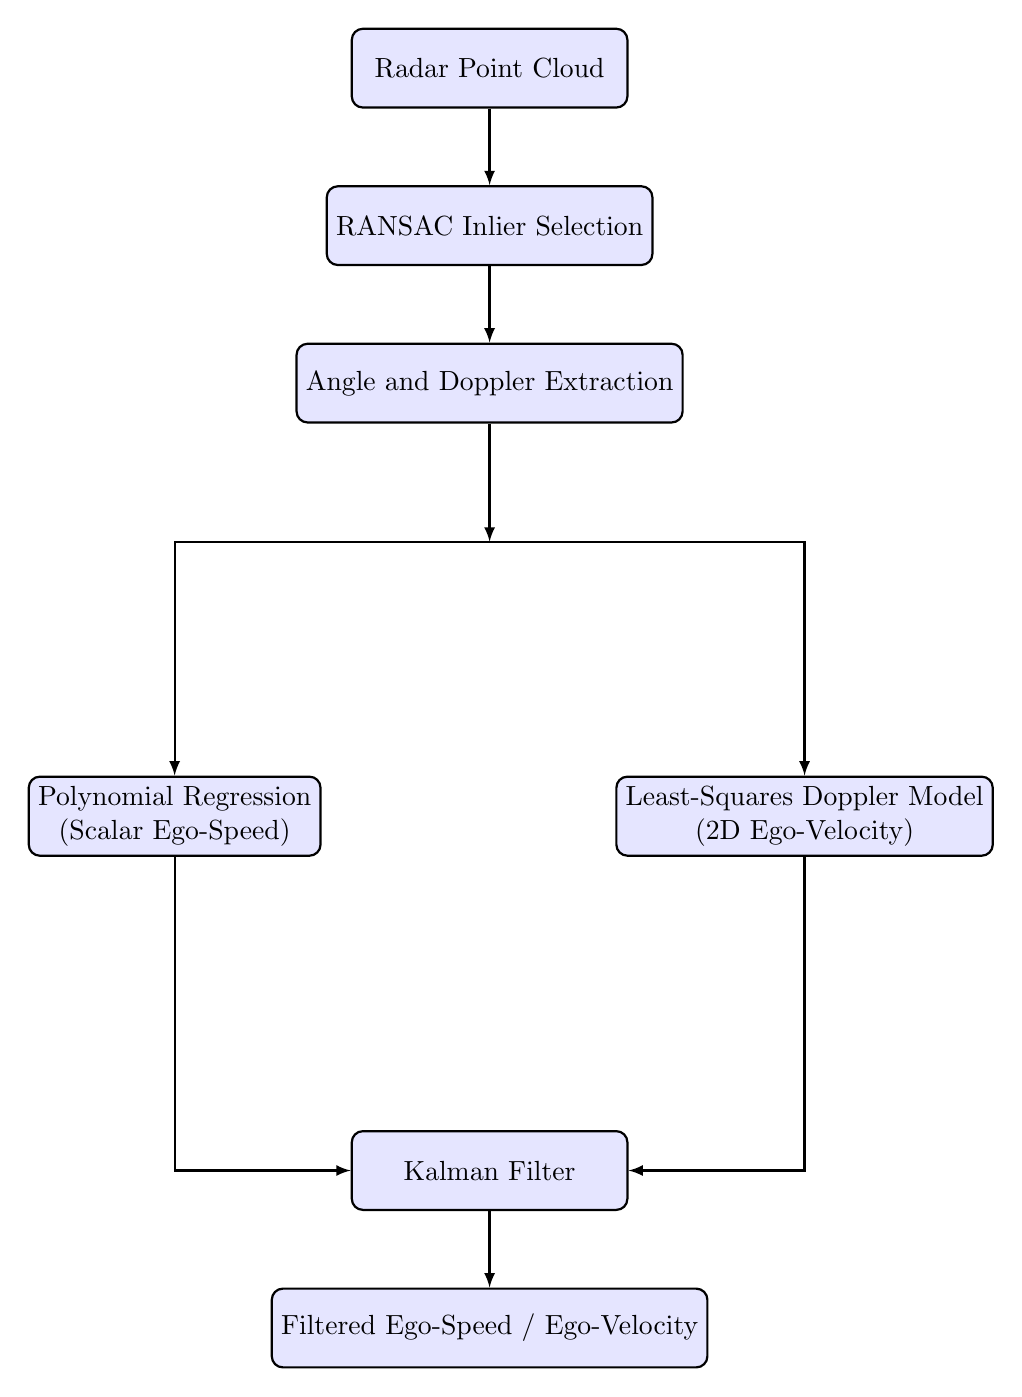
\begin{tikzpicture}[node distance=2cm,>=latex,thick]
        \tikzstyle{block} = [rectangle, draw, fill=blue!10, text centered, rounded corners, minimum height=1cm, minimum width=3.5cm, align=center]
        \tikzstyle{arrow} = [->, thick]

        % Nodes
        \node[block] (input) {Radar Point Cloud};
        \node[block, below of=input] (ransac) {RANSAC Inlier Selection};
        \node[block, below of=ransac] (angles) {Angle and Doppler Extraction};

        % Branch nodes
        \node[block, below of=angles, xshift=-4cm, yshift=-3.5cm] (scalar) {\shortstack{Polynomial Regression \\ (Scalar Ego-Speed)}};
        \node[block, below of=angles, xshift=4cm, yshift=-3.5cm] (vector) {\shortstack{Least-Squares Doppler Model \\ (2D Ego-Velocity)}};

        % Output and filter
        \node[block, below of=angles, yshift=-8cm] (kalman) {Kalman Filter};
        \node[block, below of=kalman] (output) {Filtered Ego-Speed / Ego-Velocity};

        % Straight arrows
        \draw[arrow] (input) -- (ransac);
        \draw[arrow] (ransac) -- (angles);

        % Branching arrows (down, then sideways)
        \draw[arrow] (angles.south) -- ++(0,-1.5) coordinate(branch);
        \draw[arrow] (branch) -| (scalar.north);
        \draw[arrow] (branch) -| (vector.north);

        % Merge arrows (sideways, then down)
        \draw[arrow] (scalar.south) |- (kalman.west);
        \draw[arrow] (vector.south) |- (kalman.east);

        % Final output
        \draw[arrow] (kalman) -- (output);
    \end{tikzpicture}
    \caption{Block diagram of the self-speed estimation process, showing the two complementary approaches: scalar polynomial fitting and 2D Doppler-based least-squares estimation.}
    \label{fig:self_speed_block}
\end{figure}


\subsection{Kalman Filter}
The Kalman filter is a widely used mathematical algorithm to improve the accuracy of measurements by reducing the noise and uncertainty inherent in sensor data. This is done via estimations of what could be the next state using prior measurements to obtain this "next" state. 
To enhance the accuracy of the self-speed estimation, a 1D Kalman (meaning that it is used to estimate only one state) filter was implemented.
This filter estimates the vehicle's exact velocity based on the provided radar-based seld speed estimation data.
\begin{figure}[!htbp]
    \centering
    \includegraphics[width=1.0\linewidth]{images/kalman_2.jpg}
    \caption{Kalman filter prediction of the state using estimations. From: \cite{mathworks_kalman}.}
    \label{fig: Kalman filter prediction of the state using estimations.}
\end{figure}
\FloatBarrier\noindent

The Kalman filter follows a classical predict-update model, focusing on a single state variable: the vehicle’s velocity. The process and measurement uncertainty are encapsulated in the following variables:
\begin{itemize}
    \item Process variance Q: models the uncertainty in the vehicle’s motion (e.g., acceleration changes, jitter).
    \item Measurement variance R: represents the uncertainty in each self-speed estimation sample.
\end{itemize}

Where in real life the implementation can be represented as:
\begin{itemize}
    \item Estimated value: the current velocity estimate.
    \item Estimated error: the uncertainty (variance) of the current estimate.
\end{itemize}
At each new frame, a new self-speed estimation is used to update the Kalman filter which effects its output by a variable which is called Kalman Gain 'K':
\begin{equation}
K = \frac{\hat{P}}{\hat{P} + R}
\end{equation}
Where:
\begin{itemize}
    \item $\hat{P}$: predicted error variance
    \item $R$: measurement variance
\end{itemize}
This process allows the filter to balance trust between the incoming measurement and the current estimate. Over time, the filter becomes more confident, reducing the influence of noisy measurements.

Thus, the incorporation of the Kalman filter in this project provides smoother, more reliable self-speed estimation, which enhances the performance of the following dynamic filtering stage.

\begin{figure}[!htbp]
    \centering
    \includegraphics[width=1.0\linewidth]{images/kalman.png}
    \caption{Raw self-speed vs. self-speed after Kalman filter.}
    \label{fig: Test vehicle actual speed vs estimated speed.}
\end{figure}
\input{section/12Clustering}
\subsection{Cluster Tracking}
\label{subsec:cluster_tracking}

Once clusters have been identified, it is necessary to track them over consecutive frames to ensure temporal consistency. 
A cluster tracker assigns each detected cluster a unique identifier (ID) and maintains a history of its trajectory over time. 
This enables the system to distinguish between persistent static objects and transient detections caused by noise or dynamic obstacles.

\subsubsection*{Hits and Misses}
Each tracked cluster is updated at every frame using two indices: 
\begin{itemize}
    \item \textbf{Hit Count ($h$):} The number of consecutive frames in which the cluster has been successfully matched to a detection.
    \item \textbf{Miss Count ($m$):} The number of consecutive frames in which the cluster has failed to find a corresponding detection.
\end{itemize}

A cluster is considered \textit{active} if $m \leq M_{\text{max}}$, where $M_{\text{max}}$ is the maximum allowed misses before deletion. 
This mechanism ensures that short occlusions or temporary sensor noise do not cause immediate loss of tracks.

\subsubsection*{Geometric Association}
Let $c_t = (x_t, y_t)$ denote the centroid of a cluster at frame $t$.  
For each existing track, association with a new detection is performed by minimizing the spatial distance:

\begin{equation}
    d(c_t, c_{t+1}) = \lVert c_t - c_{t+1} \rVert_2.
\end{equation}

If a fitted motion model is available, the distance is instead evaluated relative to the predicted cluster trajectory. 
In this project, a simple line-fitting approach was applied to the history of each cluster’s centroids:

\begin{equation}
    y = m x + b,
\end{equation}

where $(m,b)$ are obtained via least-squares regression over the last $N$ centroids.  
The orthogonal distance of a new detection $(x_0, y_0)$ to this fitted line is computed as:

\begin{equation}
    d_{\perp}(x_0, y_0) = \frac{|m x_0 - y_0 + b|}{\sqrt{m^2 + 1}}.
\end{equation}

The detection is associated with the track if $d_{\perp} \leq d_{\text{max}}$, where $d_{\text{max}}$ is a configurable threshold.

\subsubsection*{Track Management}
The complete tracking procedure consists of:
\begin{enumerate}
    \item \textbf{Initialization:} If no tracks exist, each cluster spawns a new track with a unique ID.
    \item \textbf{Association:} Existing tracks are matched to current detections using the minimum distance criterion.
    \item \textbf{Update:} Matched tracks increment their hit count ($h \leftarrow h+1$), reset their miss count, and append the centroid to their history.
    \item \textbf{New Track Creation:} Unmatched detections start new tracks with fresh IDs.
    \item \textbf{Deletion:} Tracks exceeding $M_{\text{max}}$ consecutive misses are deleted.
\end{enumerate}

This process ensures that each stationary object is consistently represented by the same track ID across frames, while spurious detections are naturally filtered out.

\begin{figure}[!htbp]
    \centering
    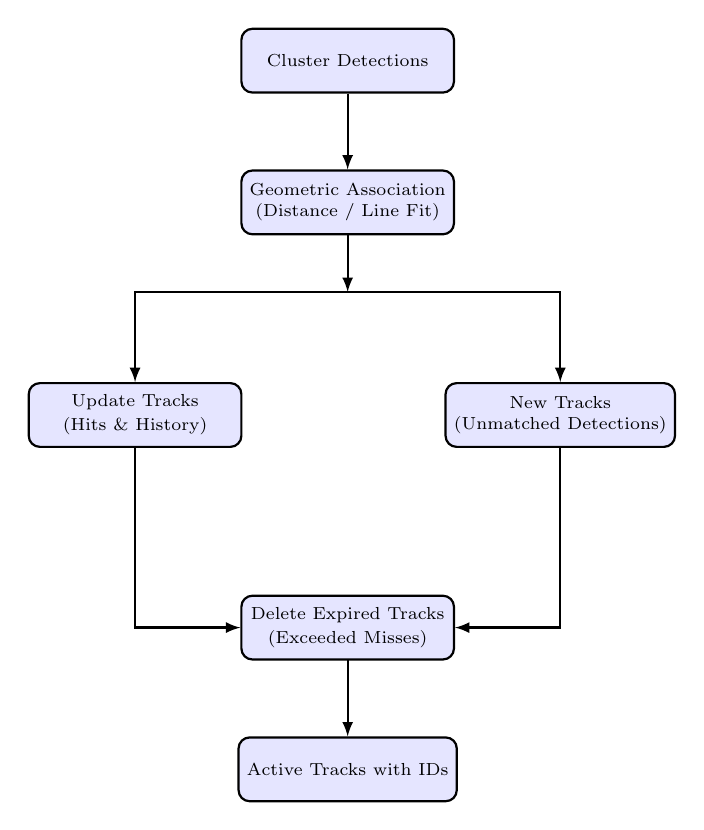
\begin{tikzpicture}[>=latex,thick,scale=0.9, every node/.style={scale=0.9}]
        % Styles
        \tikzstyle{block} = [rectangle, draw, fill=blue!10,
                             rounded corners, minimum height=0.9cm,
                             minimum width=3cm, align=center, font=\scriptsize]
        \tikzstyle{arrow} = [->, thick]

        % ==== Nodes (closer spacing, narrower width) ====
        \node[block] (input)        at (0,0)      {Cluster Detections};
        \node[block] (association)  at (0,-2)     {\shortstack{Geometric Association\\(Distance / Line Fit)}};
        \node[block] (update)       at (-3,-5)    {\shortstack{Update Tracks\\(Hits \& History)}};
        \node[block] (newtrack)     at (3,-5)     {\shortstack{New Tracks\\(Unmatched Detections)}};
        \node[block] (deletion)     at (0,-8)     {\shortstack{Delete Expired Tracks\\(Exceeded Misses)}};
        \node[block] (output)       at (0,-10)    {Active Tracks with IDs};

        % ==== Arrows ====
        \draw[arrow] (input) -- (association);

        % T-branch: down, then split left/right
        \draw[arrow] (association.south) -- ++(0,-0.8) coordinate (branch);
        \draw[arrow] (branch) -| (update.north);
        \draw[arrow] (branch) -| (newtrack.north);

        % Merge toward deletion
        \draw[arrow] (update.south) |- (deletion.west);
        \draw[arrow] (newtrack.south) |- (deletion.east);

        % Final output
        \draw[arrow] (deletion) -- (output);
    \end{tikzpicture}
    \caption{Cluster tracking block diagram. Each detection is associated with existing tracks or used to initialize new tracks. Tracks are deleted after exceeding miss thresholds.}
    \label{fig:cluster_tracking_block}
\end{figure}

To illustrate the method, Figure~\ref{fig:track_cluster_pointcloud} shows a clustered radar point cloud without temporal tracking.  
Figure~\ref{fig:track_cluster_tracked} shows the same scene after applying the tracker: each cluster is assigned an ID, along with Doppler, centroid coordinates, and hit count.  
The tracker maintains these IDs consistently across frames, enabling reliable identification of stationary obstacles.

\begin{figure}[!htbp]
    \centering
    \includegraphics[width=0.48\linewidth]{images/TrackClusterPointCloud.png}
    \includegraphics[width=0.48\linewidth]{images/TrackCluster.png}
    \caption{Illustration of the cluster tracking process. Left: clustered point cloud without tracking. Right: tracked clusters with assigned IDs, Doppler values, centroids, and hit counts.}
    \label{fig:track_cluster_pointcloud}
\end{figure}

\vspace{10\baselineskip}
\subsection{Iterative Closest Point (ICP)}
\label{subsec:icp}

The Iterative Closest Point (ICP) algorithm is a classical method for estimating rigid-body transformations between two point sets. 
In the context of radar odometry, ICP provides a way to align consecutive frames of radar point clouds in order to estimate ego-motion. 
The main goal is to determine the relative rotation $R \in SO(2)$ and translation $t \in \mathbb{R}^2$ that minimize the alignment error between a source point cloud $P = \{p_i\}_{i=1}^N$ and a target point cloud $Q = \{q_j\}_{j=1}^M$.

\subsubsection*{Mathematical Formulation}
The ICP algorithm can be separated into two main steps: correspondence search and transformation estimation.

\paragraph{Correspondence Search.}
For each point $p_i \in P$, the closest point in $Q$ is selected according to the Euclidean distance:
\begin{equation}
    q^*_i = \arg \min_{q_j \in Q} \lVert p_i - q_j \rVert_2.
\end{equation}
This step establishes a set of tentative correspondences $\{(p_i, q^*_i)\}$ between the two frames. 
Efficient implementations use spatial data structures such as KD-trees to accelerate nearest-neighbor searches.

\paragraph{Transformation Estimation.}
Once correspondences are found, the rigid-body transformation $(R,t)$ is estimated by minimizing the least-squares error:
\begin{equation}
    E(R,t) = \sum_{i=1}^{N} \lVert p_i - (R q^*_i + t) \rVert^2.
\end{equation}
The optimal solution can be obtained using singular value decomposition (SVD) of the cross-covariance matrix between the two point sets. 
In 2D, the rotation can be parameterized by an angle $\theta$, such that:
\begin{equation}
    R(\theta) = 
    \begin{bmatrix}
        \cos\theta & -\sin\theta \\
        \sin\theta & \cos\theta
    \end{bmatrix}.
\end{equation}

The transformation is then applied to $Q$, and the process is repeated iteratively until convergence, typically when changes fall below a threshold or a maximum number of iterations is reached.

\subsubsection*{Global ICP}
In the global variant, all available points of the radar point cloud are used to compute correspondences and estimate the motion. 
This maximizes the use of sensor information but can be sensitive to noise and dynamic objects, since outliers directly affect the transformation estimate.

\subsubsection*{Cluster-wise ICP}
To increase robustness, a cluster-wise approach was also investigated. 
Instead of using the entire point cloud, correspondences are restricted to clusters identified in the previous stage (see Section~\ref{subsec:cluster_tracking}). 
Among these clusters, priority is given to those with the highest \emph{hit count} and lowest \emph{miss count}, since they are more likely to represent stable, stationary objects. 
For each cluster $C_k$, an independent ICP alignment is performed:
\begin{equation}
    E_k(R,t) = \sum_{p_i \in P_k} \lVert p_i - (R q^*_i + t) \rVert^2,
\end{equation}
where $P_k$ and $Q_k$ denote corresponding cluster subsets across two consecutive frames.
The resulting transformations are then aggregated, typically via weighted averaging based on cluster stability, to obtain the final ego-motion estimate.

\subsubsection*{Practical Considerations}
Several practical aspects influence ICP performance:
\begin{itemize}
    \item \textbf{Initialization:} ICP assumes small inter-frame motion. Poor initialization may cause convergence to local minima.
    \item \textbf{Nearest-neighbor search:} KD-trees enable efficient correspondence search in $\mathcal{O}(N \log N)$ time.
    \item \textbf{Outlier rejection:} Correspondences with distances exceeding a threshold $d_{\max}$ are discarded to reduce the influence of spurious points.
    \item \textbf{Cluster selection:} Restricting ICP to stable clusters improves robustness against moving objects and noise.
\end{itemize}

\subsection{Iterative Closest Point (ICP) for Ego-Motion Estimation}
\label{subsec:icp}

The Iterative Closest Point (ICP) algorithm estimates the rigid-body transformation 
between two consecutive radar frames. Given two point sets
\[
P = \{p_i \in \mathbb{R}^2 \}_{i=1}^{N}, \quad
Q = \{q_j \in \mathbb{R}^2 \}_{j=1}^{M},
\]
the goal is to find a rotation $R \in SO(2)$ and translation $t \in \mathbb{R}^2$ that minimize the alignment error
\[
\min_{R,t} \sum_{i=1}^N \lVert R p_i + t - q_{\pi(i)} \rVert^2,
\]
where $\pi(i)$ denotes the index of the nearest neighbor of $p_i$ in $Q$.

\subsubsection*{Nearest Neighbor Matching}
To associate points between frames, a KD-tree was constructed over the set $Q$.  
For each point $p_i \in P$, its closest match $q_{\pi(i)}$ is obtained as:
\[
\pi(i) = \arg\min_j \lVert p_i - q_j \rVert_2.
\]

\subsubsection*{Per-Point Motion Estimates}
For each matched pair $(p_i, q_{\pi(i)})$, the incremental translation and orientation change are computed as
\[
t_i = p_i - q_{\pi(i)}, \qquad
\theta_i = \arctan2\!\left( (p_i - q_{\pi(i)})_y, (p_i - q_{\pi(i)})_x \right).
\]

\subsubsection*{Global Averaging}
The global motion is obtained by averaging over all matched pairs:
\[
\bar{t} = \frac{1}{N} \sum_{i=1}^N t_i, \qquad
\bar{\theta} = \frac{1}{N} \sum_{i=1}^N \theta_i.
\]

\subsubsection*{Homogeneous Transformation Matrices}
The estimated transformation from ICP is expressed in homogeneous coordinates as:
\[
T_{\text{ICP}} =
\begin{bmatrix}
\cos\bar{\theta} & -\sin\bar{\theta} & \bar{t}_x \\
\sin\bar{\theta} &  \cos\bar{\theta} & \bar{t}_y \\
0 & 0 & 1
\end{bmatrix}.
\]

For ego-motion estimation (inverse motion), the corresponding matrix is:
\[
T_{\text{ego}} =
\begin{bmatrix}
\cos\bar{\theta} & \sin\bar{\theta} & -(\bar{t}_x \cos\bar{\theta} + \bar{t}_y \sin\bar{\theta}) \\
-\sin\bar{\theta} & \cos\bar{\theta} & \;\;\bar{t}_x \sin\bar{\theta} - \bar{t}_y \cos\bar{\theta} \\
0 & 0 & 1
\end{bmatrix}.
\]

\subsubsection*{Cluster-wise ICP}
In addition to the global ICP (using all points), a cluster-wise ICP is applied.  
Each cluster $C_k$ maintains counters for \emph{hits} and \emph{misses}, ensuring stable targets are prioritized.  
For each cluster, the transformation $(t_k, \theta_k)$ is estimated using the above procedure.  
The global motion estimate is then computed as a weighted average:
\[
\bar{t} = \frac{\sum_k w_k t_k}{\sum_k w_k}, \qquad
\bar{\theta} = \frac{\sum_k w_k \theta_k}{\sum_k w_k},
\]
with weights
\[
w_k = \max\!\left(\min\!\left(\text{hits}_k^{\alpha}, \; \text{max\_hits}\right), 1\right),
\]
where $\alpha \in [1,2]$ controls the influence of stable clusters.

\subsubsection*{Python-style Conceptual Flow}
\begin{enumerate}
    \item Input two frames $P$ and $Q$.
    \item Use a KD-tree to find nearest neighbors between $P$ and $Q$.
    \item For each matched pair $(p_i,q_{\pi(i)})$, compute translation $(t_x,t_y)$ and rotation $\theta$.
    \item Average all translations and rotations to obtain $(\bar{t},\bar{\theta})$.
    \item Build the homogeneous transformation $T_{\text{ICP}}$.
    \item Derive the inverse ego-motion matrix $T_{\text{ego}}$.
    \item (\textbf{Cluster ICP}) Repeat steps 2–6 on each cluster and fuse results using hit-based weighting.
\end{enumerate}

\section{Summary and Outlook}

Insert conclusion here
%\section{WIP - Storing TikZ graphics}

\begin{figure}[!htbp]
    \centering
    \resizebox{0.48\textwidth}{!}{
        \begin{tikzpicture}
            % Block styles
            \tikzstyle{block} = [rectangle, draw, text width=4.5em, text centered, minimum width=6em, minimum height=4em]
            \tikzstyle{block_dashed} = [rectangle, draw, text width=2em, text centered, minimum width=4em, minimum height=4em, dashed]
            % Input and output
            \node[block, right=of antenna, minimum width=4em, minimum height=4em] (frames) {Frames};
            \node[block, right=of frames] (frame_aggr) {Frame\\Aggregator};
            \node[block, right=of frame_aggr] (coord_filter) {Filter\\$x,y,z$\\$\phi,SNR$};
            \node[block, right=of coord_filter] (self_speed_estim) {Self-speed Estimator};
            \node[block, right=of self_speed_estim] (self_speed_kalman) {Kalman Filter};
            \node[block, below=of self_speed_estim] (ve_speed_calc) {Calculation\\of $v_{e}$};
            \node[block, right=of ve_speed_calc] (ve_filter) {Filter\\$v_{e}$ vs. self-speed};
            \node[block, right=of ve_filter] (clustering) {Clustering};
            % Connections
            \draw[->] (frames) -- (frame_aggr); % Connection from antenna to RF amplifier
            \draw[->] (frame_aggr) -- (coord_filter);
            \draw[->] (coord_filter) -- (self_speed_estim);
            \draw[->] (coord_filter.south) |- (ve_speed_calc.west);
            \draw[->] (self_speed_estim) -- (self_speed_kalman);
            \draw[->] (self_speed_kalman) -- (ve_filter);
            \draw[->] (ve_speed_calc) -- (ve_filter);
            \draw[->] (ve_filter) -- (clustering);
        \end{tikzpicture}
    }
    \caption{Block diagram of the pipeline}
    \label{fig:block_diag_pipeline}
\end{figure}

\begin{figure}[!htbp]
    \centering
    \resizebox{0.48\textwidth}{!}{
        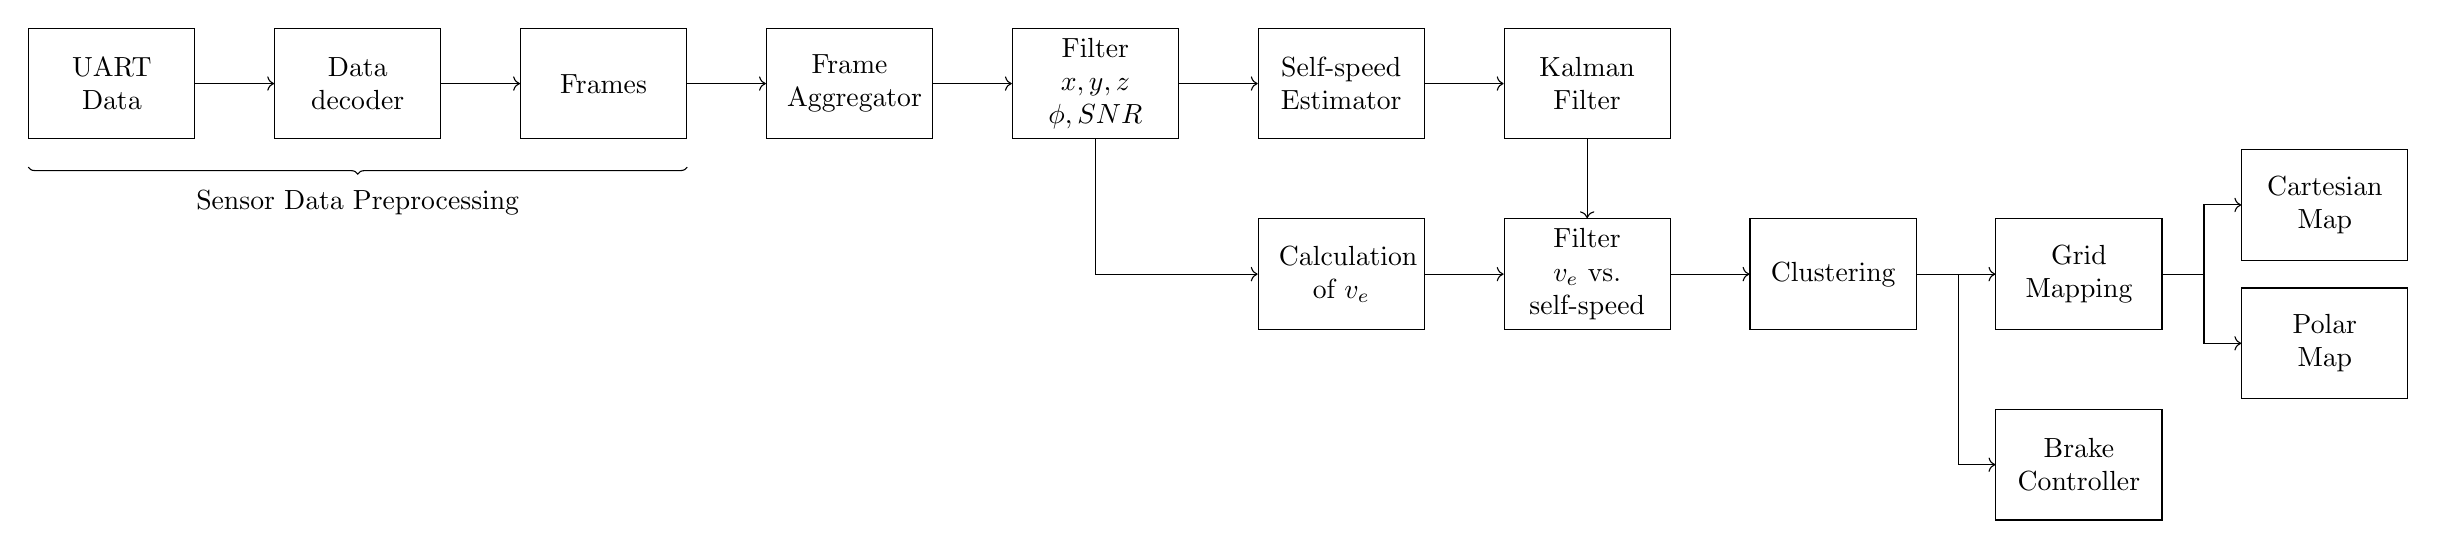
\begin{tikzpicture}
            % Block styles
            \tikzstyle{block} = [rectangle, draw, text width=4.5em, text centered, minimum width=6em, minimum height=4em]
            \tikzstyle{block_dashed} = [rectangle, draw, text width=2em, text centered, minimum width=4em, minimum height=4em, dashed]
            % Input and output
            \node[block] (uart) {UART\\Data};
            \node[block, right=of uart] (decoder) {Data decoder};
            \node[block, right=of decoder] (frames) {Frames};
            \node[block, right=of frames] (frame_aggr) {Frame\\Aggregator};
            \node[block, right=of frame_aggr] (coord_filter) {Filter\\$x,y,z$\\$\phi,SNR$};
            \node[block, right=of coord_filter] (self_speed_estim) {Self-speed Estimator};
            \node[block, right=of self_speed_estim] (self_speed_kalman) {Kalman Filter};
            \node[block, below=of self_speed_estim] (ve_speed_calc) {Calculation\\of $v_{e}$};
            \node[block, right=of ve_speed_calc] (ve_filter) {Filter\\$v_{e}$ vs. self-speed};
            \node[block, right=of ve_filter] (clustering) {Clustering};
            \node[block, right=of clustering] (grid_mapping) {Grid Mapping};
            \node[block, right=of grid_mapping.east, yshift=2.5em] (grid_cartesian) {Cartesian\\Map};
            \node[block, right=of grid_mapping.east, yshift=-2.5em] (grid_polar) {Polar\\Map};
            \node[block, below=of grid_mapping] (brake) {Brake\\Controller};
            % Connections
            \draw[->] (uart) -- (decoder);
            \draw[->] (decoder) -- (frames);
            \draw[->] (frames) -- (frame_aggr); % Connection from antenna to RF amplifier
            \draw[->] (frame_aggr) -- (coord_filter);
            \draw[->] (coord_filter) -- (self_speed_estim);
            \draw[->] (coord_filter.south) |- (ve_speed_calc.west);
            \draw[->] (self_speed_estim) -- (self_speed_kalman);
            \draw[->] (self_speed_kalman) -- (ve_filter);
            \draw[->] (ve_speed_calc) -- (ve_filter);
            \draw[->] (ve_filter) -- (clustering);

            \draw[-] (clustering.east) --++(1.5em, 0) coordinate (arrw_clustering);
            \draw[->] (arrw_clustering) -- (grid_mapping);
             \draw[->] (arrw_clustering) |- (brake);

            \draw[-] (grid_mapping.east) --++(1.5em, 0) coordinate (arrw_mapping_grids);
            \draw[->] (arrw_mapping_grids) |- (grid_cartesian.west);
            \draw[->] (arrw_mapping_grids) |- (grid_polar);

            \draw [decorate, decoration = {brace, mirror, raise=10pt}] (uart.south west) --  (frames.south east) node[pos=0.5,below=15pt,black]{Sensor Data Preprocessing};
        \end{tikzpicture}
    }
    \caption{Block diagram of the pipeline}
    \label{fig:block_diag_pipeline}
\end{figure}


\begin{figure}[!htbp]
    \centering
    \resizebox{0.48\textwidth}{!}{
        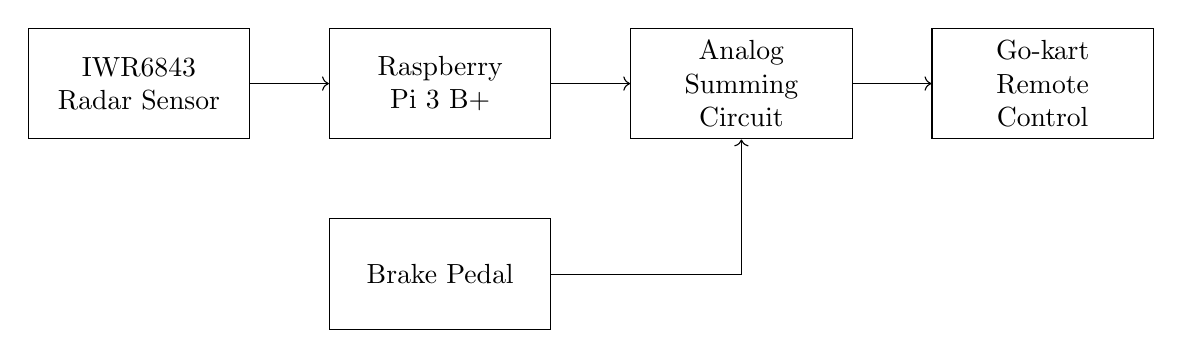
\begin{tikzpicture}
            % Block styles
            \tikzstyle{block} = [rectangle, draw, text width=6.5em, text centered, minimum width=8em, minimum height=4em]
            \tikzstyle{block_dashed} = [rectangle, draw, text width=2em, text centered, minimum width=4em, minimum height=4em, dashed]
            % Input and output
            \node[block] (radar) {IWR6843\\Radar Sensor};
            \node[block, right=of radar] (rpi) {Raspberry\\Pi 3 B+};
            \node[block, right=of rpi] (analog_summ) {Analog Summing\\Circuit};
            \node[block, below=of rpi] (brake_pedal) {Brake Pedal};
            \node[block, right=of analog_summ] (remote) {Go-kart\\Remote Control};
            % Connections
            \draw[->] (radar) -- (rpi);
            \draw[->] (rpi) -- (analog_summ);
            \draw[->] (brake_pedal) -| (analog_summ);
            \draw[->] (analog_summ) -- (remote);
        \end{tikzpicture}
    }
    \caption{Block diagram of the pipeline}
    \label{fig:block_diag_pipeline}
\end{figure}
\newpage

\begin{thebibliography}{00}

\bibitem{ninebot_product_page} Segway Inc., ``Ninebot Go-kart PRO product page'', 2025, Webpage. [Online]. Available: \url{https://de-de.segway.com/products/ninebot-gokart-pro}

\bibitem{iwr_awr_diff} Texas Instruments, ``IWR1642: difference between AWR and IWR parts'', 2025, Webpage. [Online]. Available: \url{https://e2e.ti.com/support/sensors-group/sensors/f/sensors-forum/742730/iwr1642-difference-between-awr-and-iwr-parts}

\bibitem{dev_board_page} Texas Instruments, ``IWR6843AOPEVM product page'', 2025, Webpage. [Online]. Available: \url{https://www.ti.com/tool/IWR6843AOPEVM}

\bibitem{mmwave_demo_doc} Texas Instruments, ``User's Guide mmWave Demo Visualizer,'' 2020, Online Document. [Online]. Available: \url{https://www.ti.com/lit/ug/swru529c/swru529c.pdf?ts=1742817596204}.

\bibitem{mmwave_demo_web} 
Texas Instruments, 
``mmWave Demo Visualizer'', 2025, Webpage. [Online]. Available: \url{https://dev.ti.com/gallery/view/mmwave/mmWave_Demo_Visualizer/ver/3.6.0/}

\bibitem{understanding_uart} Texas Instruments, ``Understanding UART Data Output Format'', 2025, Webpage. [Online]. Available: \url{https://dev.ti.com/tirex/content/radar_toolbox_2_20_00_05/docs/software_guides/Understanding_UART_Data_Output_Format.html}

\bibitem{mmwave_demo_output} Texas Instruments, ``mmWave Sensing Estimator'', 2025, Webpage. [Online]. Available: \url{https://dev.ti.com/gallery/view/mmwave/mmWaveSensingEstimator/ver/2.5.1/}

\bibitem{ninebot_protocol_github} ub4raf, ``Ninebot-PROTOCOL'', 2025, GitHub Repository. [Online]. Available: \url{https://github.com/ub4raf/Ninebot-PROTOCOL}

\bibitem{ninebot_protocol_scooterhacking} -, ``Ninebot ES Communicaton Protocol'', 2019, Webpage. [Online]. Available: \url{https://cloud.scooterhacking.org/release/nbdoc.pdf}

\bibitem{numpy_polyfit} -, ``numpy.polyfit documentation'', 2025, Webpage. [Online]. Available: \url{https://numpy.org/doc/stable/reference/generated/numpy.polyfit.html}

\bibitem{OccupancyGrid_Mapping_Automotive} Ç. Önen, A. Pandharipande, G. Joseph, and N. J. Myers, ``Occupancy Grid Mapping for Automotive Driving Exploiting Clustered Sparsity,'' \textit{IEEE Sensors Journal}, vol. 24, no. 7, pp. 9240-9250, 2024. [Online]. Available: \url{https://doi.org/10.1109/JSEN.2023.3342463}.

\bibitem{Odometry_radar_only}
D. Casado Herraez, M. Zeller, L. Chang, I. Vizzo, M. Heidingsfeld, and C. Stachniss, 
``Radar-Only Odometry and Mapping for Autonomous Vehicles,'' 
\textit{arXiv preprint}, 2023. [Online]. Available: \url{https://arxiv.org/abs/2305.12409}

\bibitem{EgoMotion_DopplerRadar}
S. R. Bhatt, B. S. Nadiger, R. Parthasarathy, and H. M. Shetty, 
``Instantaneous Ego-motion Estimation Using Doppler Radar,'' 
\textit{IEEE Sensors Letters}, vol. 7, no. 5, pp. 1–4, 2023. [Online]. Available: \url{https://doi.org/10.1109/LSENS.2023.3244030}

\bibitem{Multimodal_Offroad}
C. E. Beal, T. Williams, J. Pauli, M. Mukadam, and B. Boots, 
``Robust Off-Road Autonomy Using Multimodal Sensor Fusion,'' 
in \textit{Proc. of the Conference on Robot Learning (CoRL)}, 2023. [Online]. Available: \url{https://openreview.net/forum?id=kmiZqSgoAt}

\bibitem{HighSpeed_Estimation}
B. Sundaralingam, C. E. Beal, and B. Boots, 
``Robust High-Speed State Estimation for Off-Road Autonomous Vehicles,'' 
in \textit{Proc. of Robotics: Science and Systems (RSS)}, 2023. [Online]. Available: \url{https://openreview.net/forum?id=3JpFLY3ihix}


\bibitem{geeksforgeeks_dbscan}
GeeksforGeeks, 
\emph{DBSCAN Clustering in ML | Density Based Clustering}, 
2023. [Online]. Available: \url{https://www.geeksforgeeks.org/dbscan-clustering-in-ml-density-based-clustering/}. [Accessed: 19-Mar-2025].

\bibitem{mathworks_kalman}
MathWorks,
\textit{Understanding Kalman Filters, Part 3: Optimal State Estimator},
2017. Available at: \url{https://la.mathworks.com/videos/understanding-kalman-filters-part-3-optimal-state-estimator--1490710645421.html} (Accessed: March 23, 2025).

\bibitem{ti_radar_toolbox}
Texas Instruments, 
\textit{Radar Toolbox – mmWave Sensor Configuration and Demos}, 
2024. Available at: \url{https://dev.ti.com/tirex/explore/node?node=A__ADnbI7zK9bSRgZqeAxprvQ__radar_toolbox__1AslXXD__2.20.00.05} (Accessed: March 23, 2025).

\bibitem{mti710_manual}  
Movella (Xsens),  
\textit{MTi User Manual},  
2023. [Online]. Available: \url{https://www.xsens.com/hubfs/Downloads/usermanual/MTi_usermanual.pdf}. [Accessed: 26-Sep-2025].  

\bibitem{xsens_repo}  
Scottapotamas,  
\textit{Xsens MTi Device Interface and Parser},  
GitHub repository, 2020. [Online]. Available: \url{https://github.com/Scottapotamas/xsens-mti}. [Accessed: 26-Sep-2025].  

\bibitem{mti_lowlevel_doc}  
Movella (Xsens),  
\textit{Low-Level Communication Protocol Documentation},  
2023. [Online]. Available: \url{https://www.xsens.com/hubfs/Downloads/Manuals/MT_Low-Level_Documentation.pdf}. [Accessed: 27-Sep-2025].  

\bibitem{googlemaps_fhdo}
Google Maps, 
\emph{Fachhochschule Dortmund - Parking Lot Overview}, 
2025. [Online]. Available: \href{https://www.google.com/maps/search/fh+dortmund/@51.5061964,7.4567,105m/data=!3m1!1e3?entry=ttu&g_ep=EgoyMDI1MDkyOC4wIKXMDSoASAFQAw%3D%3D}{Google Maps}. 
[Accessed: 01-Oct-2025].


\end{thebibliography}


\end{document}

\begin{comment}
    [26/09/2025]
    [Guide Outline — Pre-thesis Structure]

    Abstract  
    - High-level summary: problem → method → key results → significance.  

    Introduction  
    - Background (odometry, current methods).  
    - Motivation (why radar, why this project).  
    - Research gap (what existing methods lack).  
    - Contribution statement (what you did).  

    Objectives  
    - General objective: main project goal.  
    - Specific objectives: concrete steps  
        • Design mounts  
        • Configure chirps  
        • Implement filtering pipeline  
        • Compare results  

    System Hardware  
    - Sensors (radar, IMU, webcam).  
    - Mechanical integration (3D printed mounts, placement, calibration).  
    - Chirp configuration & radar setup.  

    Methodology (Pipeline)  
    - Present the pipeline as the method.  
    - Each subsection = one module (Transformations, Frame Aggregation, RANSAC, Clustering, ICP).  
    - Show diagrams (block flowcharts, data transformations).  
    - End with summary of expected advantages of this design.  

    Implementation & Experimental Setup (Showcasing your work)  
    - Describe implementation process (code, synchronization, data collection).  
    - Explain experimental platform (Ninebot test vehicle, dual radars, IMU, lab environment).  
    - Show photos/screenshots (sensor mounts, test tracks, visualizations).  

    Results  
    - Initial results (trajectory plots, ego-speed estimation, cluster visualization).  
    - Comparison with baseline (paper approach, wheel encoder, or naive ICP).  
    - Discuss successes and limitations.  

    Discussion  
    - Interpret results: where radar odometry shines, where it struggles.  
    - How your design choices (dual radars, chirp config, RANSAC filtering) affected performance.  

    Conclusion and Future Work  
    - Wrap up contributions.  
    - Highlight possible extensions (sensor fusion, better clustering, real-world driving).  

    Bibliography  
\end{comment}
